% -*- coding: utf-8 -*-
%%
%%
%%
%%
%%
%%
%%  本模板可以使用以下两种方式编译:
%%
%%     1. PDFLaTeX
%%
%%     2. XeLaTeX [推荐]
%%
%%  注意:
%%    1. 在改变编译方式前应先删除 *.toc 和 *.aux 文件,
%%       因为不同编译方式产生的辅助文件格式可能并不相同。
%%
%%
\documentclass[12pt,openright,openany]{book}


\usepackage{ifxetex}
\ifxetex
  \usepackage[bookmarksnumbered]{hyperref}
\else
  \usepackage[unicode,bookmarksnumbered]{hyperref}
\fi

\usepackage[emptydoublepage]{NKThesis}   % 中文
%\usepackage[emptydoublepage,English]{NKThesis} % 英文

\usepackage{listings}
\usepackage{color}
\usepackage{xcolor}

\usepackage{amsmath}
\usepackage{bm}
\usepackage{amssymb}
\usepackage[ruled,vlined,algochapter]{algorithm2e}
\usepackage{subfigure}
\usepackage{multirow}
\usepackage{float}
\usepackage{booktabs}
\usepackage{fix-cm}

%   根据需要选择 biblatex 宏包选项.
%\usepackage[backend = biber, defernumbers = true,  sorting=none,  style = nkthesis]{biblatex}
\usepackage[backend = bibtex8, defernumbers = true,  sorting=none,  style = nkthesis]{biblatex}
\hypersetup{colorlinks=true,
            pdfborder=0 0 1,
            citecolor=black,
            linkcolor=black}

\raggedbottom

\addbibresource{nkthesis.bib}
\DeclareBibliographyCategory{cited}
\AtEveryCitekey{\addtocategory{cited}{\thefield{entrykey}}}

\includeonly{
abstract,
manual,
references,
acknowledgements,
resume
}
\newtheorem{Theorem}{\hskip 2em 定理}[chapter]
\newtheorem{Lemma}[Theorem]{\hskip 2em 引理}
\newtheorem{Corollary}[Theorem]{\hskip 2em 推论}
\newtheorem{Proposition}[Theorem]{\hskip 2em 命题}
\newtheorem{Definition}[Theorem]{\hskip 2em 定义}
\newtheorem{Example}[Theorem]{\hskip 2em 例}

\renewcommand\listfigurename{图清单}
\renewcommand\listtablename{表清单}
\renewcommand{\algorithmcfname}{算法}
\renewcommand\appendixname{ }

\hyphenpenalty=5000
\tolerance=1000

\newlength{\largNum}

\newlength{\tocRightMargin}
\setlength{\tocRightMargin}{2cm}

\newlength{\tocLeftMarginSecondLineFigure}
\setlength{\tocLeftMarginSecondLineFigure}{6.5em}

\makeatletter
\renewcommand*\l@figure[2]{%
  \settowidth{\largNum}{\hss #2}
  \ifnum \c@tocdepth >\m@ne%
    \addpenalty{-\@highpenalty}%
    \vskip 1.0em \@plus\p@%
    \setlength\@tempdima{3.4em}%
        \noindent%
    \begingroup
      \pretolerance=10000
      \parindent \z@ \rightskip \tocRightMargin%
      \parfillskip -\tocRightMargin%
     \leavevmode \normalsize%
     \advance\leftskip \tocLeftMarginSecondLineFigure%
      \hskip -\leftskip%
      {\figurename\mbox{\hspace{4pt}}#1}\nobreak%
       \leaders\hbox{$\m@th%
        \mkern \@dotsep mu\hbox{.}\mkern \@dotsep%
        mu$} \hfil\nobreak\hb@xt@%
                    \largNum{\hss #2}\par%
      \penalty\@highpenalty%
    \endgroup
  \fi}
\makeatother

\makeatletter
\renewcommand*\l@table[2]{%
  \settowidth{\largNum}{\hss #2}
  \ifnum \c@tocdepth >\m@ne%
    \addpenalty{-\@highpenalty}%
    \vskip 1.0em \@plus\p@%
    \setlength\@tempdima{3.4em}%
        \noindent%
    \begingroup
      \pretolerance=10000
      \parindent \z@ \rightskip \tocRightMargin%
      \parfillskip -\tocRightMargin%
     \leavevmode \normalsize%
     \advance\leftskip \tocLeftMarginSecondLineFigure%
      \hskip -\leftskip%
      {\tablename\mbox{\hspace{4pt}}#1}\nobreak%
       \leaders\hbox{$\m@th%
        \mkern \@dotsep mu\hbox{.}\mkern \@dotsep%
        mu$} \hfil\nobreak\hb@xt@%
                    \largNum{\hss #2}\par%
      \penalty\@highpenalty%
    \endgroup
  \fi}
\makeatother

\setcounter{secnumdepth}{3}

\newfontfamily\monaco{Monaco}
\begin{document}

%  设置基本信息
%  注意:  逗号`,'是项目分隔符. 如果某一项的值出现逗号, 应放在花括号内, 如 {,}
%
\NKTsetup{%
  论文题目(中文) =面向大规模网络的VoIP流量实时识别研究,
  副标题         = ,
  论文题目(英文) = A real-time identification system for VoIP traffic in large-scale networks,
  论文作者       = 王荣康,
  学号           = 2120160423,
  指导教师       = 张建忠  教授,
  申请学位       = 工学硕士,
  培养单位       = 计算机与控制工程学院,
  学科专业       = 计算机科学与技术,
  研究方向       = 网络与信息安全,
  中图分类号     = ,
  UDC            = ,
  学校代码       = 10055,
  密级           = 公开,
                   % 公开 | 限制 | 秘密 | 机密, 若为公开, 不填以下三项
  保密期限       = ,
  审批表编号     = ,
  批准日期       = ,
  论文完成时间   = 二〇一九年五月,
  答辩日期       = ,
  论文类别       = 学历硕士,
                   % 博士 | 学历硕士 | 硕士专业学位 | 高校教师 | 同等学力硕士
  院/系/所       = ,
  专业           = ,
  联系电话       = ,
  Email          = ,
  通讯地址(邮编) = ,
  备注           = ,
  是否批准为非公开论文 =,}

% -*- coding: utf-8 -*-

%\clearpage
%\addcontentsline{toc}{chapter}{摘要}
\begin{zhaiyao}
近年来,VoIP应用凭借其丰富的服务和低廉的价格已经成为了重要的通信服务手段。
%VoIP是一种把语音整合到IP协议中并通过因特网传输的网络技术,其最大的优势便是提供通过互联网和全球用户终端互联的环境。
不幸的是,VoIP服务为人类带来便利性的同时,也造成了诸多的社会问题。诈骗分子利用VoIP所提供的便利的服务实施犯罪活动,
%通过将VoIP呼叫系统架设于境外代理服务器,以匿名接入的方式对中国境内电话进行批量呼叫实施诈骗。VoIP服务基于网络技术的本质所提供的可编程性,使得诈骗分子可以修改主叫号码,操作路由跳板,
对我国诈骗案件的侦破造成了极大的困难。
%根据《2017中国反通讯网络诈骗半年报》显示,我国每15个人当中就有一个接到过诈骗电话。
我国反VoIP作案面临严峻的局势,为了使VoIP进一步服务于人类,对恶意VoIP的监管是必要的。

网络流量识别是一个较热门的研究领域,主流的流量分类方法包括基于端口的识别方法,基于字节、字符等的模式识别方法,基于行为的分析方法和基于机器学习的识别方法等。由于VoIP应用具有加密和P2P特性,以上分类方法大部分很难单独应用于VoIP流量识别,目前较为成熟的VoIP流量识别方法普遍采用多种方法结合的策略。另一方面,VoIP流量识别要求较高的实时性,一些基于流特征进行识别的方法不能被应用于实时识别。此外,对VoIP流量建立特征集的任务也是极其繁琐的。
%但是对VoIP流量的识别普遍要求要高的实时性,基于流特征的识别方法不能被应用于实时识别。而基于机器学习的识别方法需要人为的对VoIP应用建立特征集,其任务是极其繁琐的。

本文针对上述问题进行研究,第一,系统地归纳了各类VoIP识别方法,包括非实时的识别和实时的识别方法,并且从不同的识别层面上作出比较;第二,本文围绕VoIP应用类型采用CLNN(卷积神经网络,长短期记忆网络)模型提取特征,提取特征的过程不但不需要人为参与,并且提取的特征具有更高的精确度。第三,基于本文提出的方法,我们设计并实现了一个VoIP实时识别系统,该系统采用Apahce Storm作为流处理计算引擎,支持在大规模的网络中采集并识别VoIP流量。实验结果表明,该系统可以实时的准确识别VoIP流量。
\\
\end{zhaiyao}

\begin{flushleft}
\begin{guanjianci}
VoIP;流量识别;实时;卷积神经网络;长短期记忆网络
\end{guanjianci}
\end{flushleft}

%\clearpage
%\addcontentsline{toc}{chapter}{Abstract}
\begin{abstract}
Recently, owing to the service and price advantage, VoIP has become an important communication technology. 
%VoIP is a network technology that borns for the delivery of voice communications over Internet Protocol (IP) networks, the biggest advantage of VoIP is to provider the environment that supports terminals interconnect with Internet. 
Unfortunately, while providing convenience services, it also causes some social tragedies. Swindlers handle VoIP services provided by VoIP to carry out criminal activities, 
%they set up VoIP proxy server oversea and make fraud calls anonymously. Swindlers can change call ID and route hops through the programmability VoIP services provide, 
which causes great difficulties in solving fraud cases. We are facing severe situation to against VoIP frauds, in order to make VoIP applications serve humans better, it is important to keep VoIP applications under supervision. 

Traffic identification has been an active research topic in the past decade, several methods have been given, which can be generalized as port-based, pattern recognition, behavioral analysis, machine learning methods. Due to the encryption and P2P characteristics of VoIP applications, the above identification methods are difficult to be applied to VoIP traffic identification alone, researchers generally adopt a combination of several methods. On the other hand, VoIP identification has strict real-time requirements, the methods based on flow features are not applicable to real-time identification. It is troublesome to extract features for VoIP traffic.

Firstly, various VoIP identification methods are summarized and we compare them from different identification levels; Secondly, we adopt CNN(Convolutional Neural Networks) to extract features for accurate VoIP application identification. These extracted features are not only more reliable than the features extracted by humans, but also greatly improve the identification efficiency; Thirdly, we design a real-time identification system with Apache Storm, it can capture VoIP traffic in a large-scale network and identify their application types with the features we trained. The evaluation results verify that our system can identify VoIP traffic timely and accurately.
\\
\end{abstract}

\begin{flushleft}
\begin{keywords}
VoIP; application identification; real-time; CNN; LSTM
\end{keywords}
\end{flushleft}

\tableofcontents
% -*- coding: utf-8 -*-

\chapter{引言}

\section{研究背景}
近年来,VoIP(Voice Over Internet Protocol)技术发展迅速。VoIP是一种语音通信技术,可提供网际协议作为媒介进行语音传输的环境。包括智能手机、计算机和VoIP电话在内的各类终端可在蜂窝网络、Wi-Fi和以太网等各种网络环境中进行语音通信。与传统的公共交换电话网络(Public Switched Telephone Network,PSTN)相比,VoIP服务具有低通话成本、低建设成本、高扩展性、服务丰富等优势,因此,VoIP很快获取了人们的青睐。此外,公共交换电话网络可以通过FXO语音网关接入VoIP网络,从而实现两种网络之间的上下车应用,各种各样的VoIP应用也应运而生。

VoIP服务在创造大量社会价值的同时,也造成了诸多的社会问题。来自通信欺诈管制协会的报告显示,电信欺诈所造成的损失以每年29\%的速度增长。其发布的一份报告显示,2017年仅与VoIP PBX(专用交换机)相关的黑客攻击行为所造成的价值损失就高达19.4亿美元~\supercite{cfca}。据估算,每年因VoIP欺诈事件所造成的全球总损失达300-500亿美元。在国内,VoIP欺诈案件普遍表现为金融诈骗,诈骗分子利用VoIP所提供的改号服务冒充证券银行相关工作人员实时金融诈骗。诈骗分子通过将VoIP呼叫系统架设于境外代理服务器,以匿名接入的方式对中国境内电话呼叫实施诈骗。VoIP所提供的服务允许诈骗分子修改主叫号码,操作路由跳板,对我国诈骗案件的侦破造成了极大的困难。由中国信息通信研究院发布的《信息通信行业防范打击通讯信息诈骗白皮书》显示,2016 年全国共立通讯信息诈骗案件63万起,上半年造成经济损失80.4亿元~\supercite{caict}。《2017年中国反通讯网络诈骗报告》显示,每16个用户中就超过一个收到了诈骗电话~\supercite{2017}。另一方面,VoIP因其加密性而难以追踪经常被恐怖组织所利用。早在2005年,时代周刊就指出Skype为大规模技术盲点。2008年,英国每日邮报报道,阿富汗境内的塔利班恐怖武装使用Skype逃避军情六处的侦查~\supercite{dailymail}。2012年,印度时报报道,伊斯兰恐怖组织虔诚军已经开发了自己的VoIP网络Ibotel用以躲避侦查~\supercite{timesofindia}。

为应对以上问题,各国都对VoIP技术有不同程度的监管。在我国,对IP业务牌照审核有严格的要求,实行适度开放VoIP业务的政策。这也意味着未经授权的VoIP业务是非法的,并且所有合法的VoIP业务也必须处于监管之下以应对任何程度的紧急情况。但是随着技术的进步,越来越多的VoIP应用开始采用加密和对等网络的方式,甚至有一些大型厂商采用自己的VoIP协议,这些都使得VoIP识别任务愈发艰难。大数据时代的到来为VoIP识别提供了新的思路,VoIP数据规模的增加使得越来越多的信息可供挖掘和分析,通过所挖掘的信息识别VoIP流量。本文将结合深度学习和大数据处理技术,对大规模网络中的VoIP流量进行实时识别,以支撑网络管理员对非法VoIP流量进行监管。

%加图

\section{研究现状}
在过去的十几年内,网络流量分类一直是一个研究热点。同时因为VoIP技术的发展,针对VoIP的网络流量分类吸引了很多研究者,许多有价值的工作也随之产生。

同其他流行的应用一样,早期的VoIP应用也使用由IANA(The Internet Assigned Numbers Authority,互联网数字分配机构)所指定的端口号。但是随着P2P和NAT技术的发展,许多厂商开始在自己的VoIP软件中使用这两项技术,VoIP应用不再局限于使用固定端口号,而是采取动态端口映射的方案。这就使得传统的基于端口号的识别方法不再有效。为了克服这种困难,一些研究人员\supercite{14, 16}通过识别某些特定协议如SIP,RTP协议所携带的特征来进行VoIP流量识别。一些研究\supercite{18}则从应用级别的角度对VoIP应用采取DPI(Deep Packet Inspection,深度包检测)的方式提取相关特征进行VoIP识别。这些识别方法仅仅可以识别分析过的VoIP应用,不可能做到对更多VoIP应用的识别,并且这种方式对于Skype这种私有协议是无效的。其次,这些方法不能识别采用了加密技术的VoIP应用。

\begin{table} [thb]
\caption{IANA指定的VoIP默认端口}\label{tab:21}
\small
\centering
%[t]
{
\begin{tabular}{cccc}
  \toprule
        VoIP协议 & 端口 & 传输层协议 \\
  \midrule
        SIP & 5060 & TCP/UDP \\
        SIPS & 5061 & TCP/UDP \\
        SIP Audio & 2326-2485 & UDP\\
        H.323 & 1300, 1718-1720 & TCP/UDP\\
        H.323 Audio & 2326-2485 & UDP\\
        MGCP & 2427 & TCP/UDP\\
        MEGACO/H.248 & 2944, 2945 & TCP/UDP\\
 \bottomrule
\end{tabular}
}
\end{table}

基于统计分析的方法是另一种经常被用于检测VoIP流量的方法。诸如数据流的包长度、包到达间隔、持续时间和分组交换率等统计特征被分析用于检测VoIP流量\supercite{2}。一些研究方法\supercite{19}结合流的统计特征分析和主机行为估计方法,通过设置参数D用于过滤非VoIP的流量,之后通过EL(large inter-packet time,最大包到达间隔)和ES(small inter-packet time,最小包到达间隔)计算出的参数R再次准确的识别VoIP流量。与此同时,一些最新的研究\supercite{20,21}仍然在采用基于规则和统计分析的方法检测VoIP流量。这些方法需要根据对应的规则设置很多的阈值参数,越来越多的VoIP应用会导致这些阈值参数有很大的出入。随着机器学习技术的发展,基于统计分析的方法也被赋予了新的生命力。一些研究\supercite{5}提出了使用机器学习的方法识别加密的VoIP流量。他们建立了基于流的特征集并且使用了3中机器学习的方法来训练数据集,3中机器学习方法有不错的识别率,其C5.0获得了最优的效果。机器学习的方式减轻了研究人员在设定阈值方面的负担,但是终归还是基于统计分析的方法,并且对于更新速度越来越快的VoIP应用来说,每种VoIP应用都可能在短时间内更新自己的算法,这样就需要认为的重新进行统计分析来适应VoIP的更新。尤其中作者提出的方法是基于整个VoIP数据流训练数据集,训练所得的分类器并不适用于实时的VoIP流量识别。从流量识别级别的角度来说,上述方法大多应用于检测VoIP流量,也就是说,仅仅针对VoIP流量与非VoIP流量进行识别,不能从应用级别的角度进行识别。

VoIP流量识别最大的难点是要求更高的实时性,一些研究也从实时识别的角度进行VoIP识别的研究工作。为了实时的检测VoIP流量,数据包长度在60-150字节内的UDP数据包将会被判断成VoIP数据包\supercite{3}。在这篇文章中,作者仅仅致力于提高VoIP的服务质量,该方法不追求较高的识别率所以不能被应用于准确的VoIP实时识别。一种基于VoIP会话熵变和解编码器类型的方法被提出\supercite{4},文章考虑了几种流行的VoIP应用并研究了它们的解编码器类型,通过解编码器类型可以初步的识别一些VoIP应用。为了更加准确的识别VoIP应用,他们研究了N个连续数据包之间的长度关系,并且用熵来衡量它们之间的异质性,通过解编码器类型和熵的异质性来识别VoIP流量。从实时识别的角度,他们采取了具有N个长度的滑窗计算这N个数据包的异质性,通过识别N个数据包就可以识别整个流的VoIP应用类型。相同的实时识别策略也被文章\supercite{22}采纳,作者通过提取整个双向流的前几个数据包的PSD(Packet Size Distribution,包长分布)用于识别VoIP应用,实验结果显示这种方式可以在双向流建立之后立即识别出VoIP应用类型。目前为止所有的VoIP实时识别方案都是基于识别子流的方式从而得知整个数据流的应用类型,这种方式的识别精度与所采用的滑窗大小有直接关系,采用的滑窗太小会导致识别精度太低,滑窗太大会降低实时性。尤其因为识别所采用的特征太少,文章\supercite{4}采用两个特征识别数据流,文章\supercite{22}采用一个特征识别数据流,因此识别精度不是很高。

\section{本文主要工作}

本文主要针对VoIP流量识别两个难点展开研究,研究的识别方法通用与加密和非加密VoIP应用。两个研究难点,其一是识别精度的问题,提高识别精度的根本在于寻找更加精确的特征集;其二是保证识别的实时性,提高实时性要求减少识别所需的数据包长度。本文研究了现有的VoIP流量识别的方法,并对卷积神经网络和长短期记忆网络进行了阐述。利用卷积神经网络在频域方面的建模能力和长短期记忆网络在时域方面的建模能力提取精度更高的特征集。本文针对多种VoIP应用建立数据集用于有监督的训练。综合研究成果,本文将训练所得分类器应用于实时识别系统,该系统可支撑在大规模网络中实时识别VoIP应用。

1)VoIP流量识别综述。本文对几种常用的流量识别方法进行了归纳和总结,并将其与VoIP流量识别做了比较,总结了VoIP流量识别的难点。对现有的几种VoIP流量识别方法进行了详细介绍,分析了其优缺点和适用性。

2)基于CLNN模型的VoIP识别方法。本文研究了CNN和LSTM的适用性,结合了卷积神经网络在频域方面和长短期记忆网络在时域方面的建模能力,通过研究多种网络模型设计了适用于VoIP流量的网络模型。该模型可以提取最优的特征集,避免了人工提取特征集的繁杂工作,并且具有良好的识别性能。

3)VoIP实时识别系统的实现。对CLNN模型训练所的的特征集,本文使用了4中机器学习方法重新训练分类器,这些分类器较CLNN模型具有更好的实时性。为处置大规模网络中的流量,本文采用了Apache Storm作为流式计算引擎,拓扑结构中包含多种分类器Bolt,网络管理员可以根据紧急程度采用不同的识别结果。

\section{本文的组织结构}
本文的结构安排如下:

第一章为引言,主要介绍了VoIP流量识别的研究背景和研究现状,阐述了VoIP流量识别的必要性和目前的识别方法所存在的不足,最后介绍了本文的主要研究内容。

第二章为相关研究,介绍了VoIP相关技术并比较了传统的流量识别与VoIP流量识别的异同,详细的分析了现有研究方法的适用范围和优缺点。最后,介绍了本文所采用的卷积神经网络和长短期记忆网络的基本原理。

第三章为基于CLNN网络的特征提取相关研究。该章首先分析了VoIP流量所携带的可支持识别的特征,其次介绍了本文所采用的用以支撑实时识别的方案。最后介绍了如何构建VoIP流量数据集并使用CLNN模型训练数据集提取特征集,详细介绍了CLNN模型的设计。

第四章为VoIP流量实时识别系统的实现。该章介绍了实时系统的总体框架。之后从离线训练和在线识别两个方面介绍了系统的实现。

第五章为实现结果以及性能评估。评估了CLNN模型提取的特征集,并对4种机器学习训练所得的分类器进行了评估。

第六章总结了全文的工作,分析了本文研究工作的不足之处以及进一步的研究方向。


\chapter{相关研究}
VoIP流量识别是从各种网络协议流量中识别出VoIP相关流量,并对其进一步分类的过程。VoIP流量识别主要用于保障网络安全,可以依VoIP应用类型对流量作出不同的处置。本章将首先对VoIP技术进行介绍,并从基于信令控制流量识别和媒体传输流量识别两个角度进行分析。之后介绍了两种可用于VoIP流量实施识别的方法并分析了其局限性。最后,介绍了本文使用的用于提取特征的两种神经网络结构。
%本章对多种传统流量识别方法进行了总结分析,并比较了其与VoIP流量识别的异同,介绍了VoIP识别的难点。最后详细阐述了卷积神经网络与长短期记忆网络的基本原理。

\section{VoIP简介}
VoIP(Voice over Internet Protocol,基于IP的语音传输协议)是一种网络通话技术,经由网际协议来达成语音传输,也就是在互联网上进行语音通信。早期的VoIP技术是在个人电脑上通过软件的方式实现的,当时的VoIP软件只能支持电脑与电脑之间进行通信。2000年,VoIP技术在IP PBX的加持下,开始向电信领域渗透。传统的公共交换电话网络可以通过IP PBX接入FXO网关连接到互联网,从而实现传统公共交换电话与网络电话之间的通信,这也导致了VoIP技术的飞速发展。VoIP技术发展至今,作为宽带电话已经从语音质量、价格等各个方面超越了传统的固定电话。

VoIP协议包括用于信令控制和媒体传输两方面的相关协议。主流的VoIP协议包括H.323,SIP,MGCP,MEGACO和RTP/RTCP等。其中H.323和SIP作为被广泛使用的信令控制协议主要用于呼叫建立、呼叫保持和呼叫终止,它们由不同的标准化组织制定,SIP主要用于分组网络,H.323同时用于分组网络和电路网络。MGCP和MEGACO协议在概念和结构上有很多重叠,两种协议都可以说是对H.323协议簇的进一步发展,其中MGCP定义了网关分离的思想,大幅度提高了媒体网关的可用性;MEGACO即H.248现属于H.323协议簇的一部分,建立在MGCP基础之上,其功能强大、扩展性良好,允许在呼叫控制层建立多个分区网关,已开始逐步取代MGCP。实时传输协议即RTP为语音提供端到端的传输服务,其包括RTP和RTCP两个子协议,是最主流的VoIP媒体传输协议。因为本文的VoIP识别方法主要基于对RTP/RTCP流量进行识别,本节将对信令控制协议和实时传输协议作简单。

\subsection{信令控制协议}
本节将对H.323协议簇和SIP两种信令控制协议作简单介绍,并分析信令控制协议在VoIP流量识别方面的优缺点,并解释为什么本文没有采用分析信令控制协议的方案识别VoIP流量。
\subsubsection{H.323}
H.323协议簇是于1996年由ITU-T制定针对多媒体通信的协议,它包括呼叫控制、媒体编码、管理控制、网络安全等一系列协议,是目前使用最为广泛的VoIP通信协议。本节我们主要介绍H.323协议簇的核心内容,包括H.323结构相关、H.225和H.245协议。

H.323结构中定义了多个提供多媒体通信的网络元素,这些元素包括终端、多点控制单元、网关和网守等。H.323系统中所定义的终端包括支持语音视频编解码、远程信息处理和用户界面的设备,需要支持H.323协议簇所支持的一系列协议堆栈;多点控制单元由多点控制器和多点处理器组成,用于管理多点回忆,可以进行音频混合、视频切换等操作;网关是用于分组交换网络和其他电路交换网络,如PSTN和ISDN,进行数据转换的元素;网守在H.323网络中是可选的,用于提供包括最重要的地址解析在内的多种服务,其主要通过H.225中的RAS协议实现与网关的信令传输。

H.225协议主要包括两部分的内容,RAS和Q.931。RAS协议是用于网关和网守之间的通信协议,其独立于呼叫建立和媒体传输信道,RAS一般使用1718和1719端口进行信令传输。Q.931协议用于呼叫的建立和拆除, 它使用TCP协议进行传输,一般使用端口1720建立呼叫控制信道。H.225协议中固定端口的使用是很多研究人员分析H.323协议进行VoIP流量识别的基础。

H.245协议用于建立音视频和数据传输所用的媒体传输信道,即为VoIP通话建立RTP/RTCP传输信道。它包括请求、响应、命令和指示四种类型的消息,用于协商信道使用率和功能。

%H.323协议簇作为最复杂的VoIP通信协议,除上述介绍的几个核心协议之外,还包括H.235在内的安全加密协议,多样的H.323协议簇和加密协议的存在会对我们分析H.323流量造成很大的障碍。另外,如今的H.323协议簇可以采用SSL和TLS等安全传输层协议进一步加密,从而使得H.323流量的分析更加困难。

\subsubsection{SIP}
SIP被设计用于为VoIP提供一系列扩展集调用处理功能,通过该扩展集,可以实现VoIP拨号、振铃、回铃和忙音等和传统的电话网相同的功能。SIP的设计简单、灵活、扩展性高,并且SIP最初是由IETF组织进行标准化和管理,因此它吸引了众多植根于IP标准的团体。

SIP从设计上采用了一些与HTTP相同的原则,SIP报文是人类可读的,同样采取了请求和应答的基本流程。SIP借助了很多HTTP状态码来响应请求,指示呼叫状态。SIP网络中包括多种逻辑实体,包括用户代理、代理服务器、注册服务器和重定向服务器等。其中用户代理和代理服务器用于发送请求和请求转发,注册服务器和重定向服务器用于位置注册和位置查询。图片\ref{fig:SIP}展示了SIP会话的基本呼叫流程,通话邀请请求会经过代理服务器进行转发,呼叫终止请求由用户代理之间直接发送。

\begin{figure}[thb]
\begin{center}
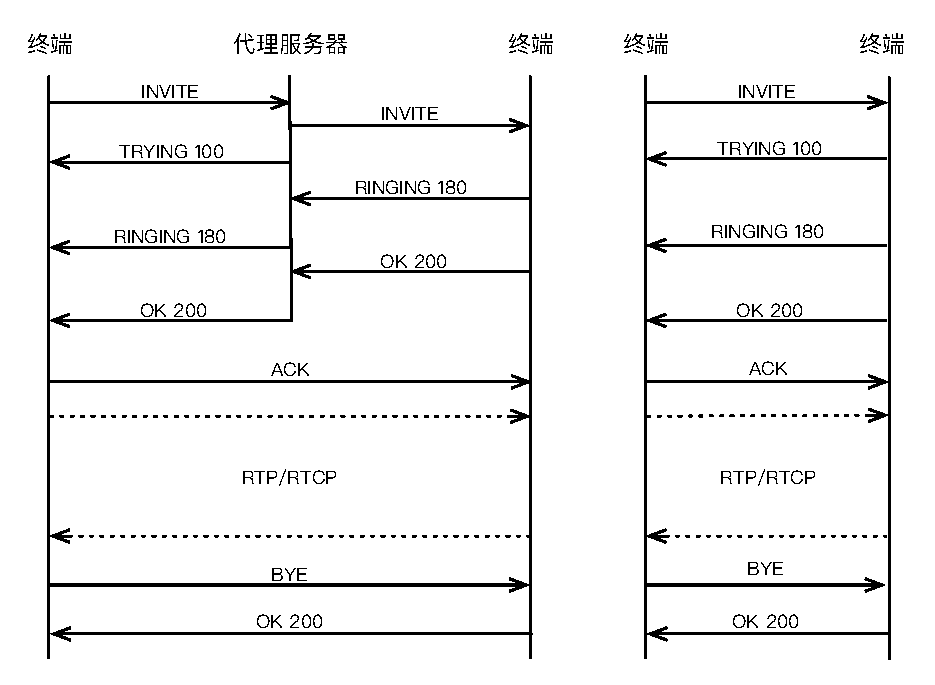
\includegraphics[width=0.8\textwidth]{figures/SIP.eps}
\caption{SIP会话连接建立基本流程}\label{fig:SIP}
\end{center}
\end{figure}

%SIP最初作为最简单的信令控制协议在VoIP通信中获得了广泛的应用。但是随之SIP技术的发展,其已经演变的和H.323一样复杂了,分析SIP请求的行为也变的越来越困难。另外,NAT技术的发展也对分析SIP行为造成了极大的困难。虽然SIP技术可以很容易的实现NAT穿越,但是NAT技术使得用于SIP请求的地址与用于RTP/RTCP媒体传输的地址不同,这就使得即使我们成功分析了SIP协议也需要重新获得用于RTP/RTCP传输的地址,对VoIP流量识别造成了新的困难。图片 展示了SIP和RTP/RTCP进行NAT穿透的过程。SIPS为SIP使用TLS提供传输安全所制定的协议,已经足够成熟被应用到各种VoIP应用。

\subsubsection{信令控制协议之于VoIP流量识别}
在VoIP发展的初期,许多研究人员通过研究信令控制协议进行VoIP流量识别。通过研究信令控制协议进行VoIP流量识别的方案仍然具有很大的价值,技术方面也具有很大的可行性。因为信令控制阶段位于媒体传输通道建立之前,所以这种方案比研究实时传输协议具有更高的实时性和完善性。

由于信令控制协议的种类纷繁复杂,研究人员都针对某一特定信令控制协议进行分析。比如对SIP进行深度包检测的研究,对H.323协议的端口进行分析,对私有VoIP协议Skype协议的握手规则进行分析。因此,对信令控制协议的研究不利于设计通用的VoIP流量识别系统。

H.323协议簇作为最复杂的开源VoIP通信协议,除上述介绍的几个核心协议之外,还包括H.235在内的安全加密协议。多样的H.323协议簇和加密协议的存在会对我们分析H.323流量造成很大的障碍。另外,如今的H.323协议簇可以采用SSL和TLS等安全传输层协议进一步加密,从而使得H.323流量的分析更加困难。SIP最初作为最简单的信令控制协议在VoIP通信中获得了广泛的应用。但是随之SIP技术的发展,其已经演变的和H.323一样复杂了,分析SIP请求的行为也变的越来越困难。从SIP加密的角度,SIPS为SIP使用TLS提供传输安全所制定的协议,已经足够成熟被应用到各种VoIP应用。协议逐渐变得复杂而灵活以及加密技术的成熟使得对信令控制协议的研究愈发困难。

各种NAT(Network Address Translation,网络地址转换)技术和NAT穿透技术的发展也对信令控制协议的分析造成了一定的难度。SIP的NAT穿透技术包括ALG、MidCom、STUN、SBC和report等,其中以架设SBC(Session Border Controller,会话边界控制器)最为常用。该技术成功解决了媒体传输通道在NAT技术中采用随机端口的问题,图\ref{fig:sbc}展示了SBC的工作过程,其中NAT服务器和SIP服务器只进行转发,不会修改SIP数据包内容,而SBC会修改SIP数据包内容并保存各地址和端口的映射表关系。

\begin{figure}[thb]
\begin{center}
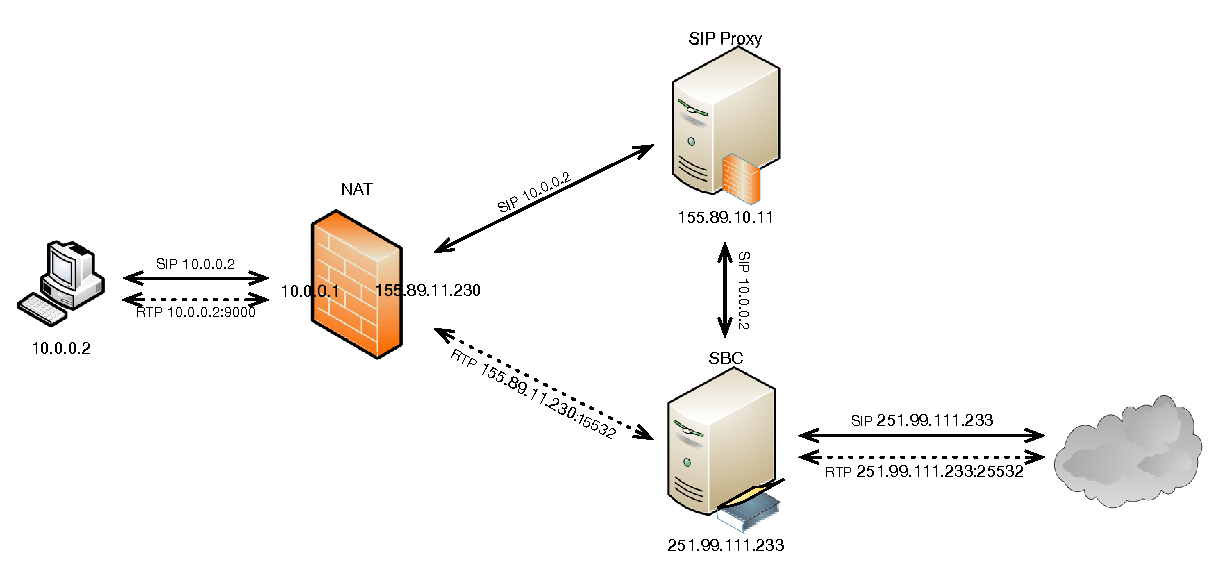
\includegraphics[width=0.9\textwidth]{figures/sbc.eps}
\caption{SBC在SIP穿透过程中的工作图示}\label{fig:sbc}
\end{center}
\end{figure}

各种软交换技术即IP PBX的发展,将传统的交换设备部件化,加之MGCP和MEGACO协议的不断完善,成功达到了呼叫控制与媒体分离的效果。这种技术在追求高性能的同时,也成功解决了授权问题、NAT穿透等诸多问题。图片\ref{fig:softswitch}展示软交换技术实现呼叫控制与媒体传输分离的基本原理。这使得研究人员即使成功的分析了信令控制协议,仍需进一步分析软交换过程确定对应的媒体传输链路。
\begin{figure}[thb]
\begin{center}
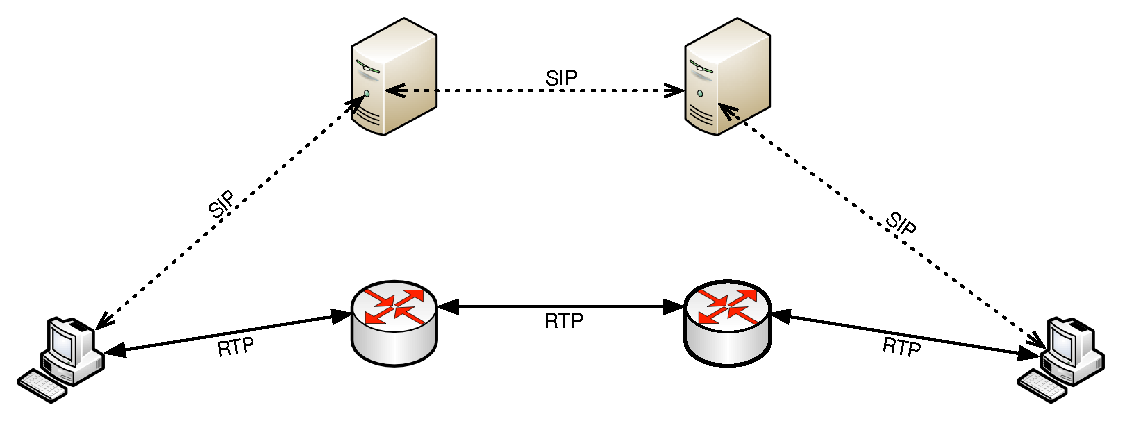
\includegraphics[width=0.9\textwidth]{figures/softswitch.eps}
\caption{软交换环境中的呼叫控制与媒体传输分离}\label{fig:softswitch}
\end{center}
\end{figure}

本文致力于找到一种方法可以应用于通用的VoIP流量识别。综上所述,由于信令控制协议的复杂、加密等的特性,对于信令控制协议的研究不适用于通用的VoIP流量识别方法。同时也由于NAT穿透技术和软交换技术的发展,造成了对信令控制协议分析的难度进一步加大,所以本文不采用信令控制协议产生的流量进行分析的方法,而是致力于使用广泛被VoIP应用采用的实时传输协议进行VoIP流量识别。

\subsection{实时传输协议}
实时传输协议(Real-time Tarnsport Protocol,RTP)普遍用于在IP网络中传输音频或视频数据。通常实时传输协议与实时传输控制协议(RTP Control Protocol,RTCP)结合使用,被广泛的应用于VoIP应用中。另外,还有用于控制流媒体服务器的实时流媒体协议(Real Time Streaming Protocol,RTSP)也经常与RTP和RTCP协议结合使用,由于RTSP本身不对流数据进行传输,主要用于控制流数据的传输,本文对RTSP不作介绍。RTP和RTCP通常采用UDP进行装载,提供端到端的实时性传输。

RTP用于装载音频和视频数据,包含了装载数据的标识符、负载类型、序列计数和时间戳等信息。图\ref{fig:rtp}展示了RTP的报头格式。我们对其中带有明显识别特征的4个占位符做简单介绍。其中M作为标记位,占1个位,对于音频负载,其标记会话的开始,对于视频负载,其标记一帧的结束。PT位标记有效负载类型,其用于通知接收该数据包的终端负载所使用的解编码器类型。如果当前终端在某种条件下需要对该数据包所包含的有效负载进行重新解编码的工作,可以按照PT位选择解编码器。由于音频负载和视频负载使用不同的解编码器,根据该位可以很容易识别出当前负载属于音频数据还是视频数据。序列号占16位,用于标识发送者所发送的RTP报文的序列号。时间戳占32位,其表示对当前数据包打包的时间。序列号和时间戳结合可以提取VoIP应用在时序方面的特征。

\begin{figure}[thb]
\begin{center}
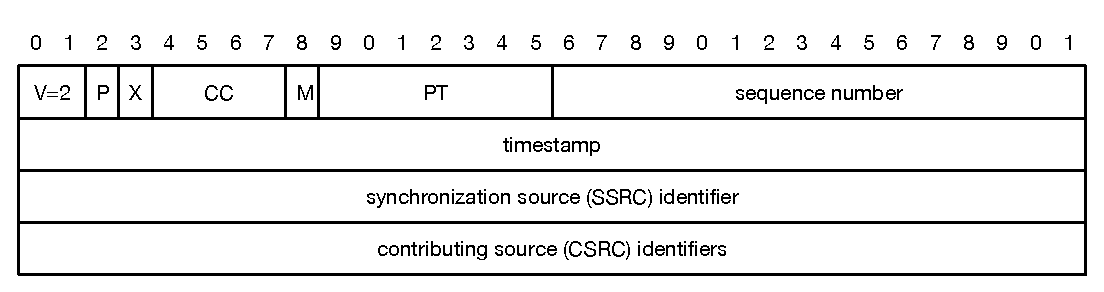
\includegraphics[width=0.9\textwidth]{figures/rtp.eps}
\caption{RTP报头格式}\label{fig:rtp}
\end{center}
\end{figure}

RTCP作为RTP的控制协议其本身并不传输数据,通常与RTP一起协作将多媒体数据打包和发送。RTCP为RTP提供质量保证服务,通过周期性的向参与者发送统计信息提供媒体分发中的服务质量的反馈信息,统计信息包括传输字节数、传输分组数、丢包数、抖动和单双向抖动延时等等。RTCP数据包具有多种不同的类型,包括RR(接收者报告包)、SR(源报告包)、SEDS(源描述包)、BYE(离开申明)和APP(特殊应用包)五类,分别用于传送不同的信息。RTCP通常使用RTP所采用的偶数端口号的下一个奇数端口号。

通过分析实时传输协议进行VoIP流量识别在识别实时性上有一定的弊端,不能像分析信令控制协议那样在建立媒体传输通道之前就可以知道通话双方即将采用的地址及端口号,并对其作出相应的措施。分析实时传输协议也有其优势,VoIP应用普遍采用实时传输协议,我们可以根据这种特点设计一套通用的VoIP识别方法。另外,VoIP应用在媒体传输阶段所产生的流量要远远多于信令控制阶段产生的流量,这一条件决定了媒体传输阶段产生的流量要有更强的识别特征。虽然这种方式在实时性上有一定的不足,但是如果在媒体传输通道建立之后的几秒钟甚至几毫秒中对其进行识别,那么在实时性方面的牺牲也是微小的。




\section{流量识别方法}
传统流量识别与VoIP流量识别有很大的差异。传统的流量识别
\subsection{传统流量识别方法}

\subsection{VoIP流量分类方法}

\section{神经网络}
为了尽最大可能的提取VoIP语音流所携带的可识别特征,本文采用了两种神经网络结构构件深度神经网络模型CLNN用于提取特征。长短期记忆网络用于提取语音流在时序方面的特征,卷积神经网络用于提取语音流在频域方面的特征。本节将对两种神经网络结构展开进行介绍。
\subsection{长短期记忆网络}
长短期记忆网络(LSTM)是一种用于提取时间序列相关关系的循环神经网络,适于处理时间序列中间隔较长的重要事件。LSTM现已被广泛的应用于各种领域,被用于执行图像识别、语音识别和自然语言处理等多种任务。本节将对LSTM从发展过程和基本原理两个方面进行介绍。
\subsubsection{发展过程}
循环神经网络(RNN)在训练过程中会出现梯度消失和梯度爆炸的现象,为了解决这一问题,S Hochreiter和J Schmidhuber于1997年提出了LSTM模型\supercite{lstm}。LSTM引入了CEC(Constant Error Carrousel)单元用于解决梯度消失和爆炸的问题,同时引入了输入输出门用于选择性的忘记和屏蔽某些输入输出,“门”的概念成功的解决了输入输出在更新权重上具有冲突的问题。以上最原始的LSTM模型具有记忆长时序列特征的特性,但是其在记忆过长的时间序列特征时,会出现LSTM细胞状态过于饱和的现象,即细胞状态对当前输入过于依赖导致失去了泛化的能力。因此,FA Gers等人在1999年针对该问题提出了遗忘门的概念\supercite{lstmforgetgate}。遗忘门可以使LSTM网络选择合适的位置进行记忆的重置,通过引入变量替换了CEC单元中的常量,解决了LSTM网络对于长时序列过于饱和的问题。FA Gers在2001年又针对LSTM细胞遗忘过多历史信息的问题引入了窥视孔连接(Peephole Connections)的概念\supercite{lstmpeephole}。这种连接是CEC单元与输入门、输出门和输出门之间的关系是双向的,增强了LSTM模型在时序上建模的能力。在LSTM不断发展的过程中,针对不同的训练任务出现了不同的版本,K Cho等人于2014年提出的GRU(Gated Recurrent Unit)是其中一个重要的版本,其在原始LSTM基础上增加了更新门,从而减小了梯度弥散的风险。如今的LSTM广泛的被谷歌、微软等公司采用执行各种任务,LSTM的发展无疑是人工智能事业发展的一大步。

\subsubsection{基本原理}
LSTM的实际结构是由单个细胞循环所组成的,细胞通过挖掘上一个时序上的输出$h_{t-1}$和当前时序上的输入$x_t$之间的关系将细胞状态由$C_{t-1}$更新为$C_{t}$。细胞内部由三个门控结构组成,分别为输入门、输出门和遗忘门。我们将介绍这三个门控结构的基本原理。

\begin{figure}[thb]
\begin{center}
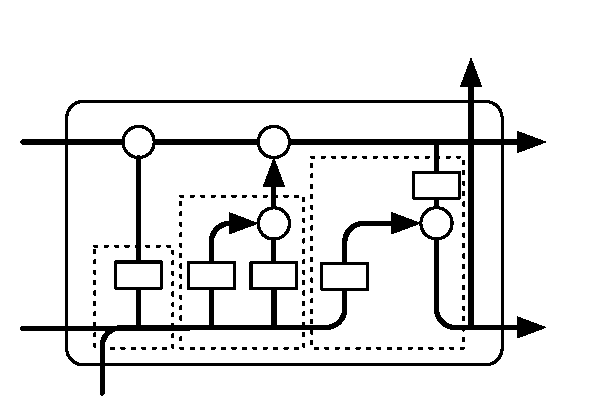
\includegraphics[width=0.6\textwidth]{figures/lstm.eps}
\caption{LSTM细胞结构}\label{fig:lstm}
\end{center}
\end{figure}

图\ref{fig:lstm}中虚线部分\textcircled{1}为遗忘门部分,遗忘门通过计算上一序列的隐藏状态$h_{t-1}$和当前序列的输入数据$x_t$之间的关系获得对上一个细胞状态$C_{t-1}$的遗忘概率$f_{t}$。数学函数表示为:
\begin{equation}
 f_t= \sigma(W_f \cdot [h_{t-1},x_t]+b_f)
\end{equation}

图\ref{fig:lstm}中虚线部分\textcircled{2}为输入门部分,输入门部分包含两个步骤,第一步是使用Sigmoid激活函数计算上一序列的隐藏状态$h_{t-1}$和当前序列的输入数据$x_t$获得本序列要更新的信息$i_t$,第二步是使用tanh激活函数计算出候选的细胞状态$\tilde C_t$。这两部分所得结果相乘即为当前序列对细胞状态更新的贡献值,再加上经过遗忘门遗忘后的细胞状态就可以获得当前序列的细胞状态$C_{t}$。数学函数表示为:
\begin{equation}
 i_t= \sigma(W_i \cdot [h_{t-1},x_t]+b_i)
\end{equation}
\begin{equation}
 \tilde C_t= \tanh(W_C \cdot [h_{t-1},x_t]+b_C)
\end{equation}
\begin{equation}
 C_t= f_t \times C_{t-1} + i_t \times {\tilde C_t}
\end{equation}

图\ref{fig:lstm}中虚线部分\textcircled{3}为输出门部分,输出门要决定在当前序列上要输出的隐藏层信息$h_t$。输出门仍然是通过使用一个Sigmoid激活函数计算上一序列的隐藏状态$h_{t-1}$和当前序列的输入数据$x_t$获得基于本序列数据的输出状态$o_t$,之后通过tanh激活函数对当前的细胞状态$C_t$处理后与输出状态$o_t$相乘,从而得到基于当前细胞状态的隐藏层信息。数学函数表示为:
\begin{equation}
 o_t= \sigma(W_o \cdot [h_{t-1},x_t]+b_o)
\end{equation}
\begin{equation}
 h_t= o_t \times tanh(C_t)
\end{equation}

经过以上三层门后,所得到的当前细胞状态$C_t$和隐藏层信息$h_t$将被用于计算下一个时序上的数据$x_{t+1}$,通过不断的更新细胞状态,细胞将会保存每个时序上最重要的信息,从而提取出时序序列在时间维度上的特征。

\subsection{卷积神经网络}
\label{sec:cnn}
卷积神经网络是一种典型的前馈神经网络,其神经元结构可以覆盖一定范围内的数据单元,有很强的在频域方面的建模能力。卷积神经网络对于二维数据有优秀的处理能力,它的网络结构所依靠的参数量也少于其他类型的网络,其被广泛的应用于视频分析、图像识别等领域。本节将对卷积神经网络的发展过程和基本原理进行介绍。
\subsubsection{发展过程}
早在1943年,WS McCulloch等人就将生物神经系统归纳为M-P神经元模型,他们的论文被认为是神经网络的开山之作\supercite{mcculloch1943logical}。K Fukushima等人在1984年提出了基于感受野的神经认知机,这是生物感受野的概念首次被应用于人工神经网络领域\supercite{fukushima1982neocognitron}。由于早期的神经网络在各个方面存在一定的局限性,神经网络的发展一直处于停滞阶段。1986年,DE Rumelhart以及GE Hinton等人提出了著名的反向传播算法\supercite{7}。在该算法受到重视的同时,神经网络的发展也迎来了第二次兴起。90年代,Y LeCun等人使用反向传播算法进行了手写数字的识别研究\supercite{lecun1990handwritten}。随后,他们又设计了一种多层的神经网络结构,取名为LeNet-5\supercite{6}。LeNet被成功应用于手写数字的分类工作,确立了CNN网络的现代结构。此时的神经网络仍受限于计算机的计算能力,在很多复杂问题上的处理结果并不理想。2012年,A Krizhevsky等人提出了一个经典卷积神经网络结构,命名为AlexNet\supercite{8}。它在2012年举办的ImageNet竞赛中获得了冠军,成功的将图片分类问题的Top5错误率降低至15\%。AlexNet在图像识别领域的成功,掀起了卷积神经网络研究的热潮。随后,K Simonyan,C Szegedy和K He等人分别设计出了VGG\supercite{9},GoogleNet\supercite{10}和ResNet\supercite{11}网络模型,它们都在各种大赛中获得了优异的成绩。值得一提的是,在各种网络通过加深神经网络层数提高识别性能时,GoogleNet模型在网络设计上做了大胆的尝试,通过引入的Inception结构在保持网络结构的稀疏性的同时也利用了密集矩阵的高计算性能。如今的卷积神经网络仍然在随着计算能力的提高而不断发展中,也已经成功被应用于医疗、金融等领域。

\subsubsection{基本原理}
卷积神经网络由输入层、隐藏层和输出层三部分组成。其中的隐藏层是卷积神经网络的核心部分,一般由卷积层、池化层和全连接层搭建而成。卷积神经网络接收多维数据作为输入,隐层中的神经元通过激活函数建立合适的权值映射到下一层中,输出即为样本对应的分类类别。本节我们对卷积神经网络的隐层部分作详细介绍。

相比于其他神经网络结构,卷积神经网络之间链接所需的参数更少。这要归功于卷积神经网络中的卷积层,其具有局部感知和权值共享两大特性。局部感知受启发于生物学里面的视觉系统结构,视觉神经元只响应某些特定区域的刺激局部的接收信息。卷积层中的神经元也没有必要对全局图像进行感知,每个神经元只需对局部状态进行感知,然后到更高层再将其感知到的信息进行综合,这样高层的神经元就具有表达全局图像状态的能力。图片\ref{fig:cnn}展示了神经元全局感知与局部感知的区别。另一方面,参数共享的特性要求图像在某一部分的特征如果和其他部分相同,在该部分学习到的特征也可以应用于其他部分上。比如我们使用$3 \times 3$的卷积核在一个部分学习到了特征,我们可以将该卷积核作为探测器应用到图像的任意其他部分,判断可不可以作为其他部分的特征的过程在反向传播中进行。卷积层可由数学函数表达为:
\begin{equation}
 a^l= \sigma(a^(l-1) * W^l + b^l)
\end{equation}
其中,a表示输入输出矩阵,l表示网络层数,W表示卷积核即权值矩阵,激活函数一般采用ReLU。
\begin{figure}[thb]
\begin{center}
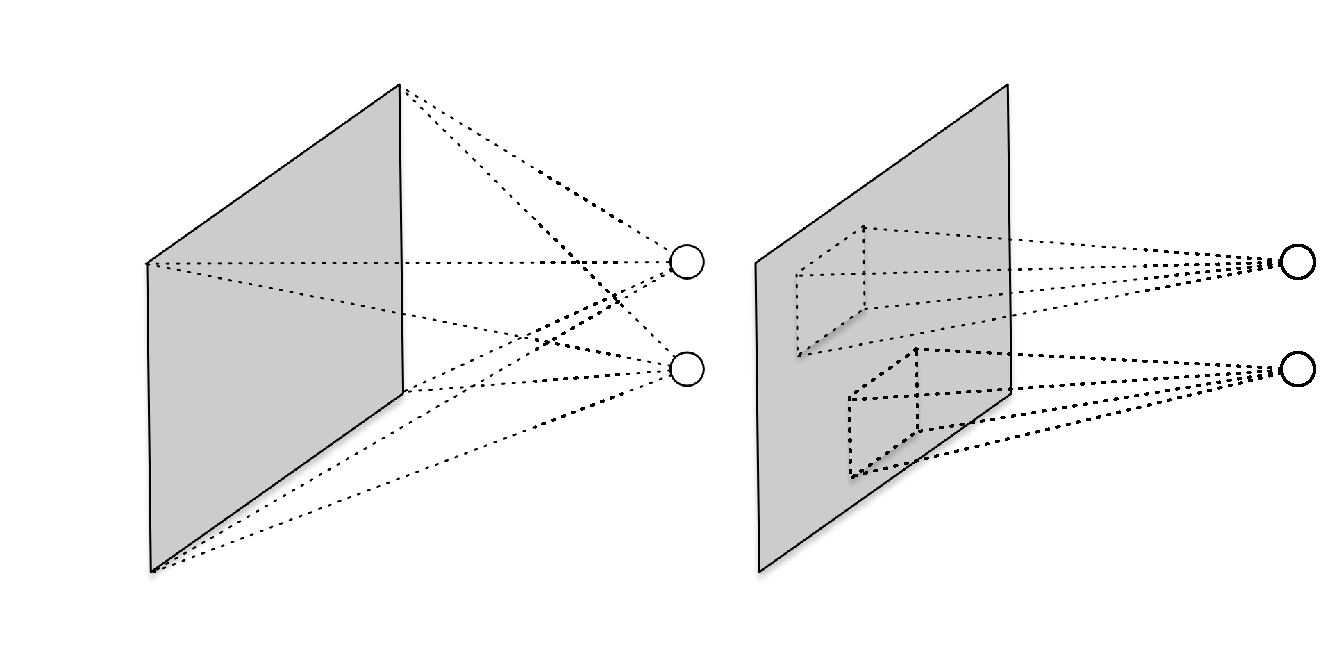
\includegraphics[width=0.8\textwidth]{figures/cnn.eps}
\caption{全局感知与局部感知}\label{fig:cnn}
\end{center}
\end{figure}

在卷积层的后面一般跟随着池化层,池化层的主要目的是进行下采样操作,下采样可以减少权值数量,在训练的过程中可以提升学习效率。常用的池化操作包括最大池化和平均池化,最大池化操作一般用于保留图像的纹理信息,平均池化操作用于保留图像的背景信息。最大池化操作对临域内的单元取最大,平均池化操作对临域内的单元取平均。如图\ref{fig:pooling}所示,池化单元大小为$2 \times 2$,步长为1。
\begin{figure}[thb]
\begin{center}
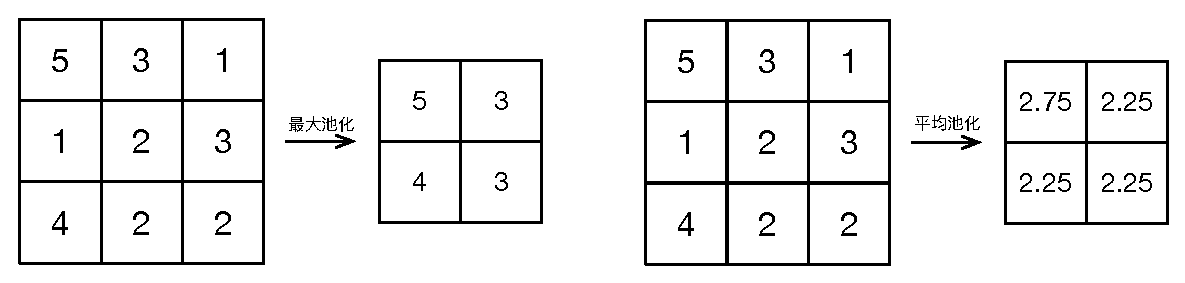
\includegraphics[width=0.9\textwidth]{figures/pooling.eps}
\caption{最大池化与平均池化}\label{fig:pooling}
\end{center}
\end{figure}

神经网络模型的输出结果一般是一维向量的形式,所以在卷积层与池化层的后方一般会进行降维操作,将多维矩阵转换为一维向量的形式输入到全连接层。全连接层实际上就是传统前馈神经网络的隐含层。通过激活函数最终映射到长度为类别种类数量的一维向量。全连接层可由数学函数表达为:
\begin{equation}
 a^l= \sigma( W^l a^(l-1)  + b^l)
\end{equation}

\subsection{长短期记忆网络与卷积神经网络}
长短期记忆网络与卷积神经网络在本质上有一定的区别,长短期记忆网络本质上属于一种循环神经网络,卷积神经网络属于前馈神经网络。图片\ref{rnn:cnn}展示了循环神经网络进行前向传播时神经元之间建立权值连接的图示,其中隐层之间在时序上建立权值连接$W$的过程是卷积神经网络所不具备的特性。长短期记忆网络擅长提取时域方面的特征,卷积神经网络擅长提取频域方面的特征,两种方法结合可以最大限度的提高VoIP流量识别的性能。

\begin{figure}[thb]
\begin{center}
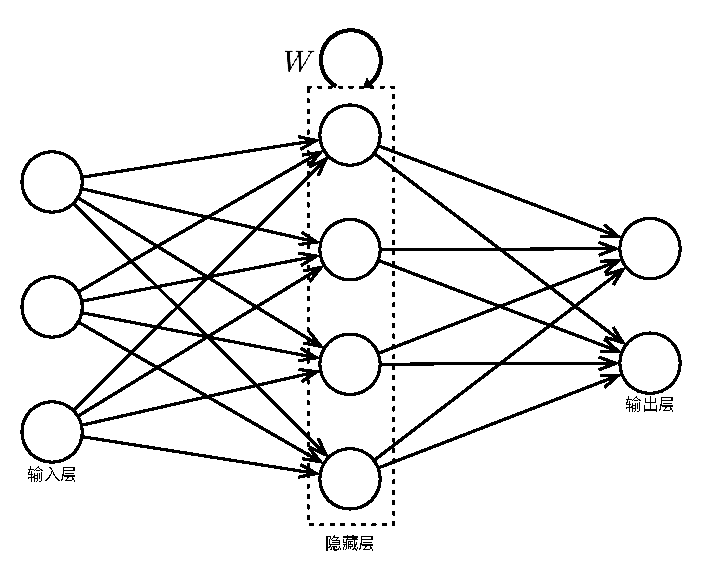
\includegraphics[width=0.6\textwidth]{figures/rnn.eps}
\caption{循环神经网络前向传播图示}\label{fig:rnn}
\end{center}
\end{figure}

长短期记忆网络与卷积神经网络在训练时都会采用反向传播算法调整权值大小,通过将正向传播计算所得的误差反向传播给隐层的神经元结构,调整隐层到输出层的权值大小。同样,输入层与隐层之间的权值也通过反向传播进行调整。反向传播算法一般使用梯度下降法,在单个样本的均方误差的负梯度方向上调节权重。

\section{本章小结}
本章主要介绍了VoIP流量识别所需的预备知识及相关研究。通过对VoIP技术的学习,分析了VoIP基于信令控制流量和媒体传输流量各自的优缺点,并基于本文的目的进行了方法的舍取。之后介绍了两种现有的VoIP流量实时识别方法并分析了其优缺点。最后,介绍了CLNN模型中采用的两种神经网络结构,并对两种结构的异同进行了介绍,指出了两种结构在特征提取方面的不同能力。






\chapter{基于CLNN模型的VoIP流量实时识别研究}
在第二章我们提到,本文针对在媒体传输阶段所产生的流量进行特征提取。第一,由于加密技术的发展,SSL/TLS,WEP和WAP/WAP2等加密技术被广泛的应用于信令控制阶段。但是由于媒体传输阶段要求更好的服务质量,考虑到加密技术需要耗费更多的计算资源,大多数VoIP应用并没有在其媒体传输阶段使用加密技术;第二,对于少量在媒体传输阶段使用机密技术的VoIP应用,因为媒体传输阶段所产生的流量要远远超过信令控制阶段,在大数据技术的支持下,媒体传输阶段的流量相比信令控制阶段可以提取更多的特征用于VoIP流量识别;第三,VoIP在信令控制阶段所采用的应用协议种类繁多,下层协议也包括UDP和TCP,而在媒体传输阶段普遍采用UDP进行传输,上层协议也普遍采用RTP进行传输,对媒体传输阶段的流量进行识别可以设计更加通用的识别方案。

%为了提取有效的特征进行VoIP流量识别,本章将从分析VoIP媒体流量所携带的特征出发,分析使用CLNN模型提取特征的可行性,进而介绍本文进行实时识别所采用的方案。并根据实时识别所采用的方案,构造用于CLNN模型训练的特征集。本章最后将会详细介绍文中设计的CLNN网络模型。

为了提取有效的特征进行VoIP流量识别,本章将从分析VoIP媒体流量所携带的特征出发,分析使用CLNN模型提取特征的可行性,进而介绍本文进行实时识别所采用的方案以及设计的CLNN网络模型。最后将会介绍本文如何使用提取的特征集进行在线实时识别。
\section{VoIP特征分析}

\subsection{基本网络特征}
RTP/RTCP是UDP的上层协议,其报头可以作为识别VoIP流量的基本网络特征。由于本文所研究的VoIP流量主要针对于语音流量。RTP中的M和PT标记位都可以作为特征用于区分视频和语音流量。RTCP在对RTP媒体传输质量提供反馈信息的同时,会根据与会者的数量调整自己的发送速率。RTP和RTCP数据包普遍采用临近端口号可以作为VoIP流量识别的另一特征。

负载类型(PT)是VoIP流量最主要的网络特征,用于指明发送端对有效负载采用的解编码器类型。由于语音在不同的通信网络中由不同的解编码器解编码,如果发送端在会话或者广播的中途决定改变编码方式,可以通过设置RTP报头中的负载类型位来通知接收端,接收端也可根据负载类型位进行解编码的工作。RTP报头中的负载类型预留位为7位,意味着RTP可以支持128种不同的负载类型。VoIP应用会在不同的网络中基于语音质量和带宽要求等相关条件选择合适的语音解编码器,每种VoIP应用所支持的语音解编码器不同。针对本文捕获的VoIP流量,表格\ref{tab:codecs}展示了我们分析所得的VoIP应用所使用的部分解编码器类型。RTP所支持的更多的负载类型可以在IANA文档\supercite{rtppt}进行查看。从解编码器的另一角度来看,不同的解编码器会使用不同的比特率传输语音,其与VoIP的各项统计特征直接相关,我们将在章节\ref{sec:statisticalfeatures}进行详细介绍。

\begin{table}[htbp]
  \caption{VoIP应用使用的解编码器}
  \label{tab:codecs}
  \centering
  \begin{tabular}{c c}
    \hline
    \textbf{应用类型} & \textbf{解编码器类型}\\
    \hline
    Skype      & dynamic (96-127), SILK, G.729, PCM A/U, GSM  \\
    UUCall      & G.723, G.728  \\
    KCCall      & PCM A/U, ILBC, GSM, G.729  \\
    Jumblo      & PCM A/U, dynamic (118)  \\
    Zoiper      & PCM A/U, GSM  \\
    Xlite      &  PCM A/U, iLBC, GSM, Speex \\
    Eyebeam      & PCM A/U  \\
    ExpressTalk      & PCM A/U, Speex  \\
    Bria      & PCM A/U, Speex, GSM  \\
    \hline
  \end{tabular}
\end{table}



\subsection{统计特征}
\label{sec:statisticalfeatures}
本节所涉及的各项统计特征都与VoIP应用所使用的解编码器类型直接相关。许多解编码器是专门为VoIP设计的,PCM A/U解编码器作为最常用的VoIP语音解编码器,这两种编码器都生成以8kHz采样的64kbps的恒定比特率(Constant Bit Rate,CBR)语音流,与其他解编码器相比可以提供较好的语音质量,但同时也较其他具有低比特率的解编码器占用更多的带宽资源。G.723和G.729作为最流行的语音解编码器,占用的带宽比较低,其中G.723支持在5.3kbps和6.3kbps两种码率下工作,G.729支持在8kbps的码率下工作。G.728也是一种使用恒定比特率的解编码器,它使用16kbps的恒定比特率运行。iLBC是对丢包具有处理能力的专为包交换网络通信设计的解编码器,优于目前流行的G.729和G.723,它可以以13.33kbps和15.20kbps的比特率工作。GSM和Speex是两种可变比特率(Variable Bit Rate,VBR)解编码器,支持宽范围的比特率,也被广泛的应用于VoIP通话技术。多数解编码器都采用20ms的打包周期,G.729采用10ms的打包周期,iLBC在13.33kbps下采用30ms的打包周期。

各种解编码器比特率和打包周期的不同,直接造成了VoIP流量所占带宽和包到达间隔的不同,同时也间接造成了数据包大小的不同。

\subsubsection{数据包大小分布}
数据包大小分布(Distribution of Packet Size,PSD)是进行VoIP流量识别最常用的统计特征。相关工作中介绍的基于PSD进行识别的研究方法直接采用PSD作为VoIP流量识别的标准\supercite{22},基于解编码器类型和熵变化的研究方法提到的数据包长度的熵变化也是数据包大小分布的表现形式\supercite{4}。

%skype DynamicRTP-Type-103
%jumblo DynamicRTP-Type-118
%xlite ITU-T G.711 PCMA
%zoiper GSM 06.10
%kc ITU-T G.729 and Comfort noise
%bria ITU-T G.711

%skype12 ITU-T G.722 与 skype013对比
%alitong ITU-T G.711 PCMU 与bria对比

%eyebeam1 ITU-T G.711 PCMU 与bria相同
%expresstalk1  ITU-T G.711 PCMU 与bria相同
图片\ref{fig:psd}中仅展示9种VoIP流量的数据包大小分布情况,其分布情况与VoIP应用所采用的解编码器有直接关系,除此之外,还与VoIP应用所选择的打包周期、解编码器的比特率以及对语音质量的不同处理有关。如图中第一行所示,Skype应用在不同的语音传输环境中会使用不同的解编码器类型,图中所示的三种解编码器在数据包大小分布上具有明显的差异。第二行展示了在采用相同解编码器情况下三种不同的VoIP应用产生的语音数据包的大小分布情况。ALT、Eyebeam和ExpressTalk三种VoIP应用都采用ITU-T G.711 PCMU解编码器,而ALT的数据包大小分布情况与其他两种有很明显的差异,Eyebeam和ExpressTalk的数据包大小分布情况很相似,可能我们不能通过数据包大小分布情况对这两种VoIP应用的流量进行识别,只能依托VoIP应用的其他特征。第三行的三种VoIP应用采用的解编码器分别为GSM、ITU-T G.729和DynamicRTP-Type-118,这三种VoIP应用所产生的流量的数据包大小分布情况与前面两行的VoIP应用同样有很大的差异。综上多种情况,VoIP应用对与不同解编码器的选择、不同比特率的选择和语音质量的保证方式都会对数据包大小分布情况产生作用,可以用作VoIP流量的识别特征。但是,同样也有很多VoIP应用在选择解编码器和比特率上作出同样的选择,所以仍需要更多的特征进行识别。

\begin{figure}[thb]
\begin{center}
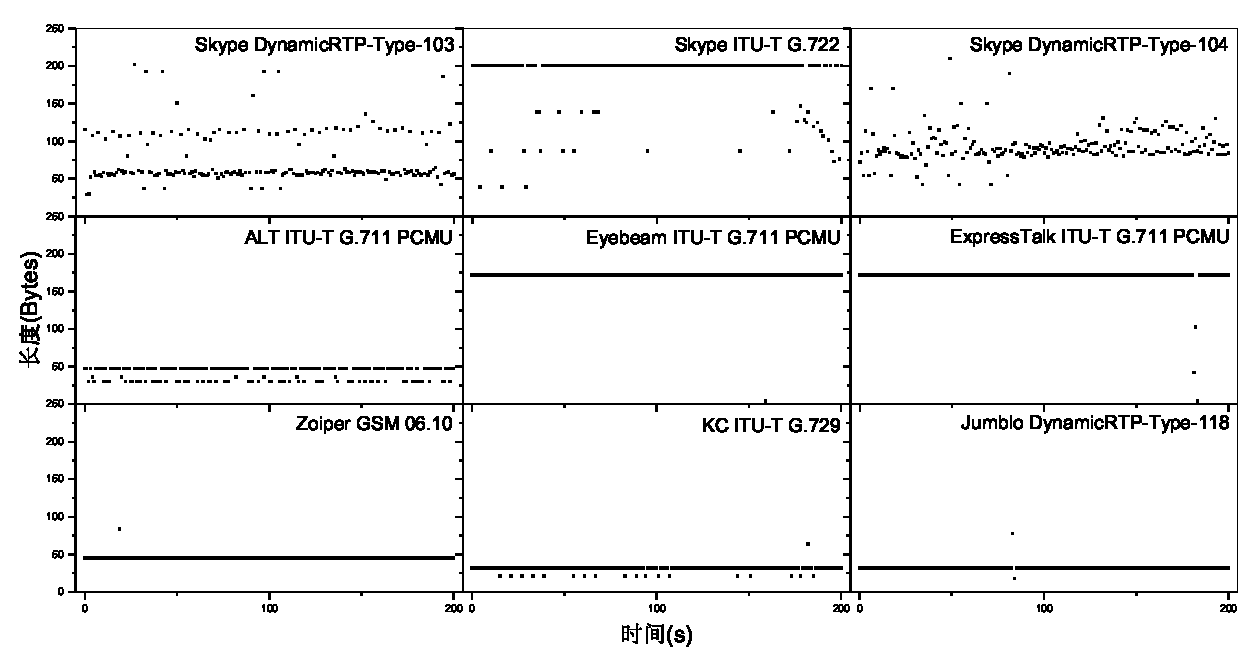
\includegraphics[width=1\textwidth]{figures/psd.eps}
\caption{数据包大小分布}\label{fig:psd}
\end{center}
\end{figure}

%图,按照\supercite{4}中的方式画

\subsubsection{包到达间隔分布}
现存的研究中很少有直接使用包到达间隔分布作为VoIP识别的特征,在一篇使用机器学习进行VoIP流分类的研究中\supercite{5},作者使用VoIP语音流的包到达间隔的标准差作为一项特征进行识别。另外,一篇进行VoIP流量统计的文章中显示,在VoIP信令控制流量和媒体传输流量中70\%的包到达间隔少于20ms\supercite{he2007analysing},意味着VoIP应用对语音的打包周期普遍少于20ms。

图中\ref{fig:itd}展示了9种VoIP应用产生的流量的包到达间隔分布。很明显的我们可以看到9种VoIP应用产生的流量的包达到间隔都有差异。具体的特征我们可以依靠深度学习方法进行提取。值得一提的是,使用数据包大小分布不能进行区分的Eyebeam和ExpressTalk两种VoIP应用的流量,此时可以通过包到达间隔分布作出区分。


\begin{figure}[thb]
\begin{center}
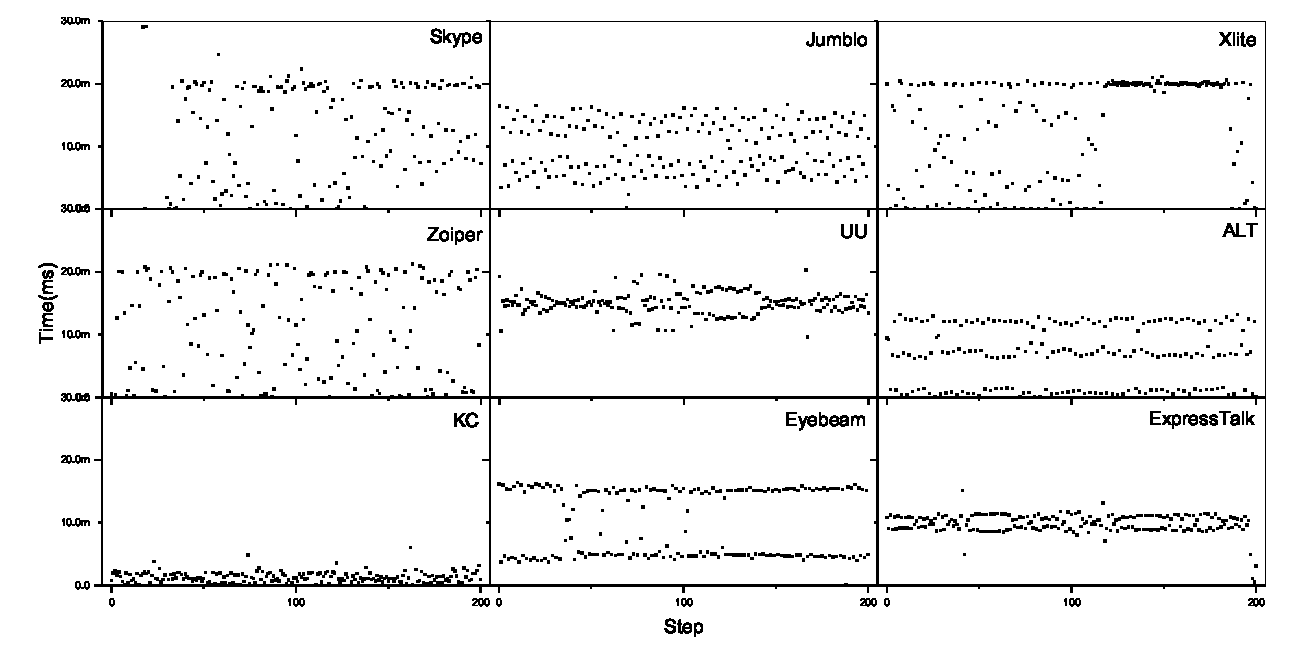
\includegraphics[width=1\textwidth]{figures/itd.eps}
\caption{包到达间隔分布}\label{fig:itd}
\end{center}
\end{figure}

\section{基于CLNN模型的特征提取研究}
\subsection{实时识别基础}
为了进行实时识别以达到流量控制的目的,可以通过在VoIP会话建立的初期识别出该VoIP会话。如果一个VoIP会话在可以接受的时间内被识别出,我们认为该识别满足了实时性的要求。假设,在一个组织内部是禁止使用某种VoIP应用的,如果我们可以在几秒钟之内准确的识别出一个VoIP流,之后在网关处拦截属于该VoIP流的全部流量,这就达到了我们实时识别的目的。

根据VoIP选择的解编码器的不同,构造并发送数据包的时间在10ms-30ms之间,这意味着VoIP应用在1秒中可以发送33-100个数据包供我们进行识别。本文将通过为VoIP子流构建数据集并提取特征集的方式,通过所提取的特征集识别VoIP子流从而确定整个流所属的应用类型。

\subsection{VoIP子流数据集构造方法}
本文采用有监督的学习方法训练数据集获取特征集,构造和标记数据集对于很多研究人员来说是一项繁琐的工作。本节我们将介绍构造适用于实时识别的带标签的数据集的方法。
\subsubsection{数据集构造}
\label{sec:construct}
数据集构造过程由收集原始数据、标记数据和拆分子流三个步骤构成。

为了获取收集原始VoIP流量,我们在真实网络环境中部署了多台电脑用于收集实验数据集。标记数据集的过程实际上是随着收集原始数据完成的,我们在Windows操作系统下采用了基于进程的流量收集工具QPA,在Linux系统下通过确定进程标识符,并按照进程标识符进行流量收集的方式。收集原始数据的过程实际上已经将原始数据按照进程名称或者进程标识符进行标记。

拆分子流的过程是将VoIP完整流拆分成多个子流的过程,我们将拆分后的单个子流叫做子流$^k$,k代表该子流中所包含的数据包个数。为了保证子流数据集的随机性,我们设计了基于滑窗的采样方法。从索引为0的数据包开始,我们采用大小为k的滑窗选择子流$^k$进入我们的数据集,滑窗的步长是在[1, k]中随机选取的。这种方式不但保证了数据集的随机性,同时也节省了大量的训练所需时间。图片\ref{fig:dataset}展示了滑窗大小为10时选择4个子流$^{10}$的过程。
\begin{figure}[thb]
\begin{center}
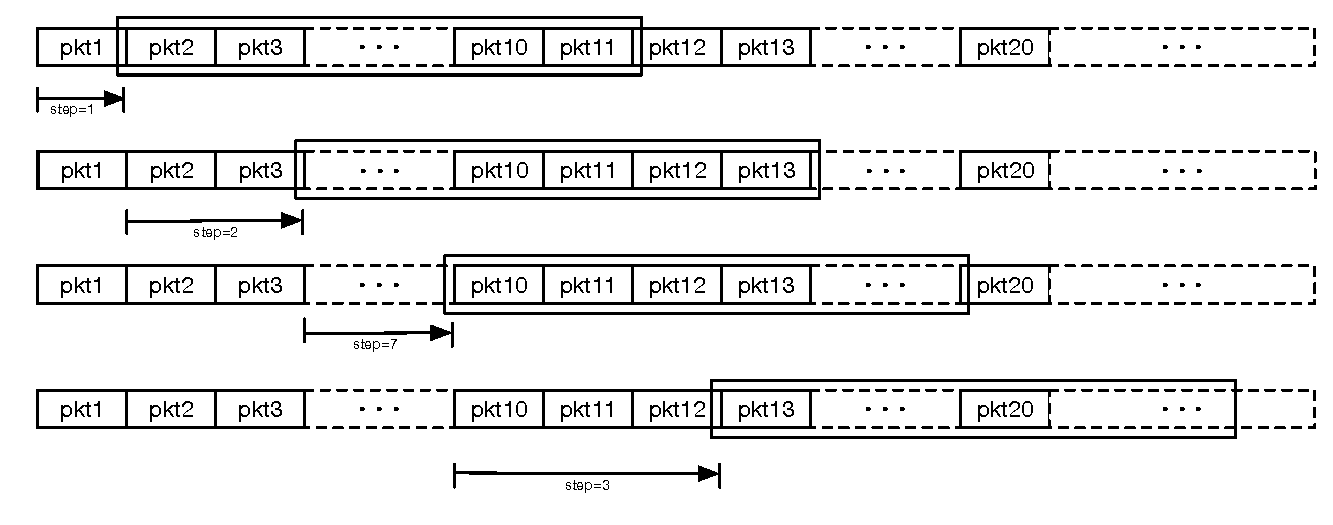
\includegraphics[width=0.9\textwidth]{figures/dataset.eps}
\caption{滑窗大小为10时选择4个子流$^{10}$}\label{fig:dataset}
\end{center}
\end{figure}

\subsubsection{数据预处理}
数据预处理的过程是将数据集处理成可供CLNN模型学习的训练数据的过程。本文提出的方法致力于识别RTP/RTCP数据流所携带的特征进而识别出VoIP流量。由于网络地址转换(Network Address Translation,NAT)技术的发展,对于我们来说,IP报头所携带的信息是没有识别价值的。UDP报头所携带的端口号信息对于我们识别RTP/RTCP数据包有一定的价值,因此我们保留UDP端口号信息。

数据预处理的过程主要包括五个步骤:1)移除网络层和传输层头部;2)为数据包添加传输层端口号;3)添加2个时间戳,一个为距离首个数据包的时间差,另一个为距离上个收据包的时间差;4)按照ASCII码将子流$^k$转换为矩阵的格式;5)对所得的矩阵进行归一化操作。根据我们的经验,RTP/RTCP数据包的长度普遍在50-210之间,因此我们将矩阵的列设为256。矩阵的行为k,即一个子流$^k$所包含的数据包个数。

\subsection{CLNN模型研究}
基于以上特征分析和构建的子流数据集,本节将介绍本文所使用的CLNN模型以及有监督学习的过程。
\subsubsection{CLNN模型结构}

我们研究了章节\ref{sec:cnn}中所提到的神经网络模型,同时吸收CLDNN模型\supercite{clnn}的设计思想设计了本文所使用的CLNN模型。正如大多数的深度学习模型,本文所使用的CLNN模型的大多数想法来自于AlexNet。唯一的不同就是我们结合LSTM和卷积神经网络两种结构中以为VoIP语音流提供更强的在时序和频域方面的建模能力。图片\ref{fig:cnnlstm}展示了CLNN模型提取VoIP子流识别特征的基本思想。使用LSTM和卷积神经网络所提取的特征将会同步被映射到全连接层,由全连接层进一步提取特征。
\begin{figure}[thb]
\begin{center}
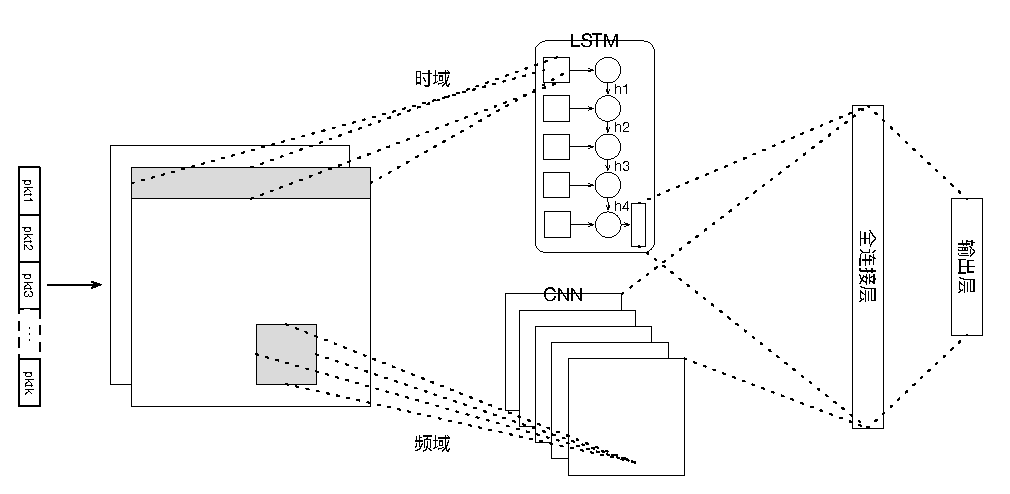
\includegraphics[width=0.9\textwidth]{figures/cnnlstm.eps}
\caption{CLNN模型提取特征的基本思想}\label{fig:cnnlstm}
\end{center}
\end{figure}
%CLNN模型由2层LSTM,3层卷积层和3层全连接层构成。

在我们的实验中,输入由大小为k$\times$l的矩阵组成,k代表子流$^k$中包含的数据包个数,l代表矩阵的列数,本文所采取的默认值为256。我们部署了两层LSTM用于提取时域上的特征,每层LSTM包含2048个细胞。平行部署了5层卷积层用于提取频域上的特征,5层卷积层所采用的参数设计基本来源于AlexNet。我们调整第一层卷积层的卷积核为5$\times$5,每层的填充类型均相同保证输入与隐层大小相同。我们在第一层卷积层后添加了最大池化层用于减少参数量,窗口大小为2$\times$2。LSTM和卷积层的输出作为隐层被连接并输入到全连接层。我们部署了3层全连接层,前两层全连接层每层具有2048个隐藏单元。第三层全连接层为输出层,使用Softmax函数进行激活,维度为11,代表样本被分到11类的概率。除LSTM和输出层外,其他各层使用ReLU作为激活函数。


\subsubsection{CLNN网络模型的学习过程}
对于CLNN模型的最后一层全连接层,我们使用Softmax作为其激活函数。在我们的实验中,一共有11中类型的流量,对于未知的VoIP流,我们通过计算其先验概率确定其应用类型。Softmax函数表示如下:
\begin{equation}
\hat P({V_i}) = softmax({V_i}) = \frac{{{e^{{V_i}}}}}{{\sum\limits_{j = 1}^n {{e^{{V_j}}}} }}
\end{equation}
其中$({V_1},{V_2},{\rm{\cdot\cdot\cdot,}}{V_i},{\rm{\cdot\cdot\cdot}},{V_n})$代表第八层的输入矩阵,$(\hat P({V_1}),\hat P({V_2}),{\rm{\cdot\cdot\cdot}},\hat P({V_i}),{\rm{\cdot\cdot\cdot}},\hat P({V_n}))$代表第八层的输出结果,它代表一个未知子流$^k$对于11中类型流量的先验概率分布,它是一个大小为$1 \times n$的向量。在我们的实验中,n为11,意味着我们的CLNN模型可以识别11中类型的流量。

在学习的过程中,我们的目标是找出最优的权值以获得最大的似然估计。寻求最大似然估计就意味着需要将多分类的对数损失函数最小化,计算损失的函数如下:
\begin{equation}
CCE({V_i}) =  - \sum\limits_{i = 1}^n {P({V_i}) \times \log (\hat P({V_i}))}
\end{equation}
其中$P({V_i})$代表${V_i}$的真实概率,它是通过训练数据集中所设置的标签所得的目标矩阵。如果j是该子流$^k$所对应的应用类型,则$P({V_j})=1$。另外的,当$i \ne j$时,$P({V_i})=0$。

在本文中,我们使用随机梯度下降(Stochastic Gradient Descent,SGD)优化器来最小化损失函数,并且在每个迭代的过程中使用牛顿动量(Nesterov Momentum)来更新梯度值。梯度增量可通过如下公式计算:
\begin{equation}
\Delta {X_t} = \tau {M_{t - 1}} - \eta \nabla f({X_{t - 1}} + \tau {M_{t - 1}})
\end{equation}
其中,${\tau}$用于表示动量因子,${\eta}$用于表示学习率。${g_t} = \nabla f({X_{t - 1}} + \tau {M_{t - 1}})$用于计算过度点的梯度,$\Delta {X_t}$表示实际下降位移,${X_t}$表示t时刻的位置,${M_t}$表示t时刻的动量。

在我们的实验中,学习率会在每轮计算后进行衰变,衰变规则如下:
\begin{equation}
\label{equ:decay}
{\eta _i} = {\eta _{i - 1}} \times \frac{1}{{1 + \rho  \times i}}
\end{equation}
其中,${\rho }$表示衰减因子,i表示当前正在进行第i轮计算。

\subsubsection{特征集}
获得更加精确的特征集用于识别VoIP流量是线下训练的目标。在我们的实验中,通过CLNN模型所提取的针对语音识别的特征集是不可读的。图片\ref{fig:feature}展示了本文CLNN模型所提取的VoIP子流的特征字节码的表现形式。尽管所提取的特征集是不可读的,我们仍然可以使用这些特征集进行其他机器学习方法的训练。本文使用所提取的特征集进行了机器学习方法的训练,并在同种条件下进行CLNN模型提取的特征集和人工提取特征集的对比实验。
%该特征集将会被用于使用SVM,random forest,decision tree和naive bayes等机器学习方法训练分类器。经过4中机器学习方法所训练的分类器均获得了较高的准确率,并且它们将会被用于我们的在线识别阶段。
\begin{figure}[thb]
\begin{center}
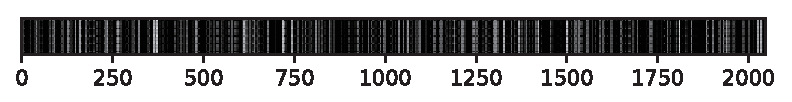
\includegraphics[width=0.9\textwidth]{figures/feature.eps}
\caption{CLNN模型所提取特征的字节码表现形式}\label{fig:feature}
\end{center}
\end{figure}

\section{在线实时识别方法研究}
\label{sec:onlineidentification}
本节将会介绍如何使用训练所得的分类器在大规模网络中进行VoIP流量的实时识别。本文包括3个主要组件用于构建我们的实时识别系统,它们分别是流量捕获器、VoIP流过滤器和分类器。流量捕获器用于捕获UDP数据包并按照IP地址和UDP端口号进行分流;VoIP流过滤器用于过滤掉明显的非VoIP流以提高系统的实时性;分类器是通过我们提取的特征集经过SVM方法训练所得,用于识别VoIP流的应用类型。

\subsection{流量捕获器}
流量捕获器维护一个待识别流数据库并且具有将捕获的数据包按照IP地址和UDP端口号分发到对应的待识别流的能力。图片\ref{fig:flow}展示了流量捕获器如何在真实网络中根据IP地址和UDP端口号分流的过程。如果刚到的数据包不能在数据库中找到对应的待识别流,流量捕获器则会使用该数据包的IP地址和UDP端口号作为键值创建一个待识别流;反之,如何可以找到对应的待识别流,则将该数据包处理后加入到该待识别流。当一个待识别流的数量达到k后,这个待识别流将会被送到下一个VoIP流过滤器组件中。


\begin{figure}[htp]
\begin{center}
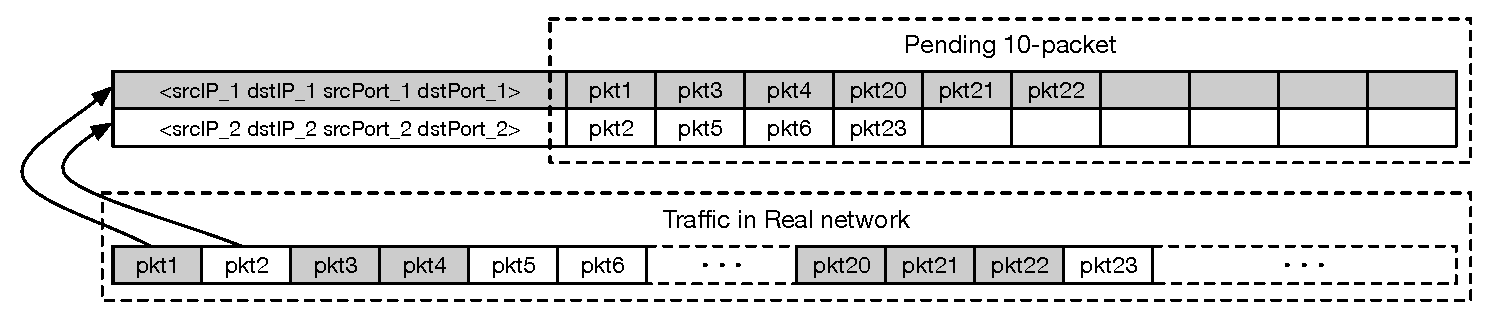
\includegraphics[width=0.9\textwidth]{figures/flow.eps}
\caption{根据IP地址和UDP端口号进行分流}\label{fig:flow}
\end{center}
\end{figure}

流量捕获器保证所捕获的数据包均为UDP数据包,并且它可以移除待识别流队列中的死流,死流是在有限时间内未达到k值的待识别流。

\subsection{VoIP流过滤器}
VoIP流过滤器作为实时识别系统的第二个重要组件,它是一个基于规则的过滤器。它接收由流量捕获器发送过来的待识别流,并对该待识别流作出初步的判断。如果初步判断的结果表明该待识别流为非VoIP流,因为非VoIP流对于我们没有任何意义,我们将不继续对该流做任何处理;如果该待识别流通过了我们设定的全部规则,则该待识别流将会被发送到分类器组件进行进一步识别。

我们从数据集中选择了一系列基准数据,并根据我们长期研究VoIP流量的经验设定了几个阈值参数用于过滤非VoIP流量。相关算法和参数分别在算法\ref{algorithm:filter}和表格\ref{tab:rules}中展示。

\begin{table}[htbp]
  \caption{算法\ref{algorithm:filter}中使用的基准值和阈值参数}
  \label{tab:rules}
  \centering
  \begin{tabular}{l l l}
    \hline
    \textbf{} & \textbf{符号} & \textbf{详细描述}\\
    \hline
    1. & min\_mpl      &   全部子流中的最小平均数据包长度\\
    2. & max\_mpl      &  全部子流中的最大平均数据包长度\\
    3. & min\_pl      &   最小数据包长度\\
    4. & max\_pl      &   最大数据包长度\\
    5. & min\_miat      &   全部子流中的最小平均包到达间隔\\
    6. & max\_miat      &   全部子流中的最大平均包到达间隔\\
    7. & min\_iat      &   最小包到达间隔\\
    8. & max\_iat      &  最大包到达间隔\\
    9. & ${\lambda_1}$, ${\lambda_2}$      &  阈值分别为上限和下限 \\
    10. & ${\varrho}$    &   比例阈值\\
    \hline
  \end{tabular}
\end{table}

%\renewcommand{\algorithmicrequire}{\textbf{Input:}}
%\renewcommand{\algorithmicensure}{\textbf{Output:}}


\begin{algorithm}[h]
\caption{用于识别VoIP/非VoIP流的算法}
\label{algorithm:filter}
\KwIn {子流$^k$}
\KwOut{VoIP/非VoIP}
\If{ ${\lambda_1}$min\_mpl $<$ 子流$^k$的平均数据包长度 $<$ ${\lambda_2}$max\_mpl \textbf{and}  ${\lambda_1}$min\_miat $<$ 子流$^k$的平均包到达间隔 $<$ ${\lambda_2}$max\_miat }{
    \For {数据包 in 子流$^k$}{
        \If{(数据包长度 $<$ ${\lambda_1}$min\_pl )}{
            $ct\_pl\_l \gets ct\_pl\_l +1$\;
        }
        \If{(数据包长度 $>$ ${\lambda_2}$max\_pl )}{
            $ct\_pl\_u \gets ct\_pl\_u+1$\;
        }
        \If{(包到达间隔 $<$ ${\lambda_1}$min\_iat )}{
            $ct\_iat\_l  \gets ct\_iat\_l+1$\;
        }
        \If{(包到达间隔 $>$ ${\lambda_2}$max\_iat )}{
            $ct\_iat\_u \gets ct\_iat\_u+1$\;
        }
    }
    \If{ct\_pl\_l $<$ ${\varrho}$k \textbf{and} ct\_pl\_u $<$ ${\varrho}$k \textbf{and} ct\_iat\_l $<$ ${\varrho}$k \textbf{and} ct\_iat\_u $<$ ${\varrho}$k}{
        \Return $VoIP$\;
    }
    \Else{
        \Return 非$VoIP$\;
    }
}
\Else{
    \Return 非$VoIP$\;
}
\end{algorithm}

\subsection{分类器}
通过VoIP流过滤器的待识别流将会被输入第三个组件分类器中,分类器所使用的特征集是在离线训练过程中经过训练所得。我们使用了4中机器学习的方法重新训练了分类器,我们将具有最好的性能的SVM分类器应用于实时识别系统。分类器将k维矩阵作为输入并输出一个大小为$1 \times n$的向量,该向量代表此待识别流可能属于每种VoIP应用的概率,最大的概率所对应的VoIP类型将作为识别结果写入数据库。与此流具有相同键值的VoIP数据包将通过查询数据库获得识别结果,供网络管理员进行下一步操作。在识别过程中,一个VoIP流会在数据包个数达到不同k值的时候被送到对应的分类器,这些分类器都会给出它们的识别结果和它们判定该流属于该识别结果的概率。

\section{本章小结}
本章首先从基本网络特征和统计特征两个角度分析了VoIP流量所携带的可供识别的特征,证明了使用媒体传输阶段所产生流量进行VoIP流量识别的可行性。之后,本章分析了进行实时识别的基本条件,并介绍了针对VoIP实时识别构建其专用的子流数据集和数据预处理的基本方法。基于以上研究,本文针对VoIP语音流量设计了在频域和时域两个方面具有良好建模能力的CLNN模型,该模型可以自动提取VoIP流量的抽象特征,在VoIP识别方面具有良好的识别性能。本章最后介绍了在大规模网络中进行实时识别的方法,介绍了实时识别系统的三个重要组件及其对应特性。















\chapter{VoIP流量实时识别系统实现}
本章根据第三章提出的基于CLNN模型进行VoIP流量识别的方法,设计并实现了一个可在大规模网络环境中进行VoIP流量识别的实时系统。本章首先对VoIP实时识别的整体框架做了介绍,之后对系统的离线训练和在线识别过程分别做了详细介绍。

\section{框架设计}
图片\ref{fig:architecture}展示了本文VoIP流量实时识别系统的总体框架。图中展示了两个阶段的具体步骤,离线训练阶段所获的的分类器作为实时识别阶段的第三个组件分类器,在实时识别阶段可以对VoIP流作出准确识别。
\begin{figure}[thb]
\centering
%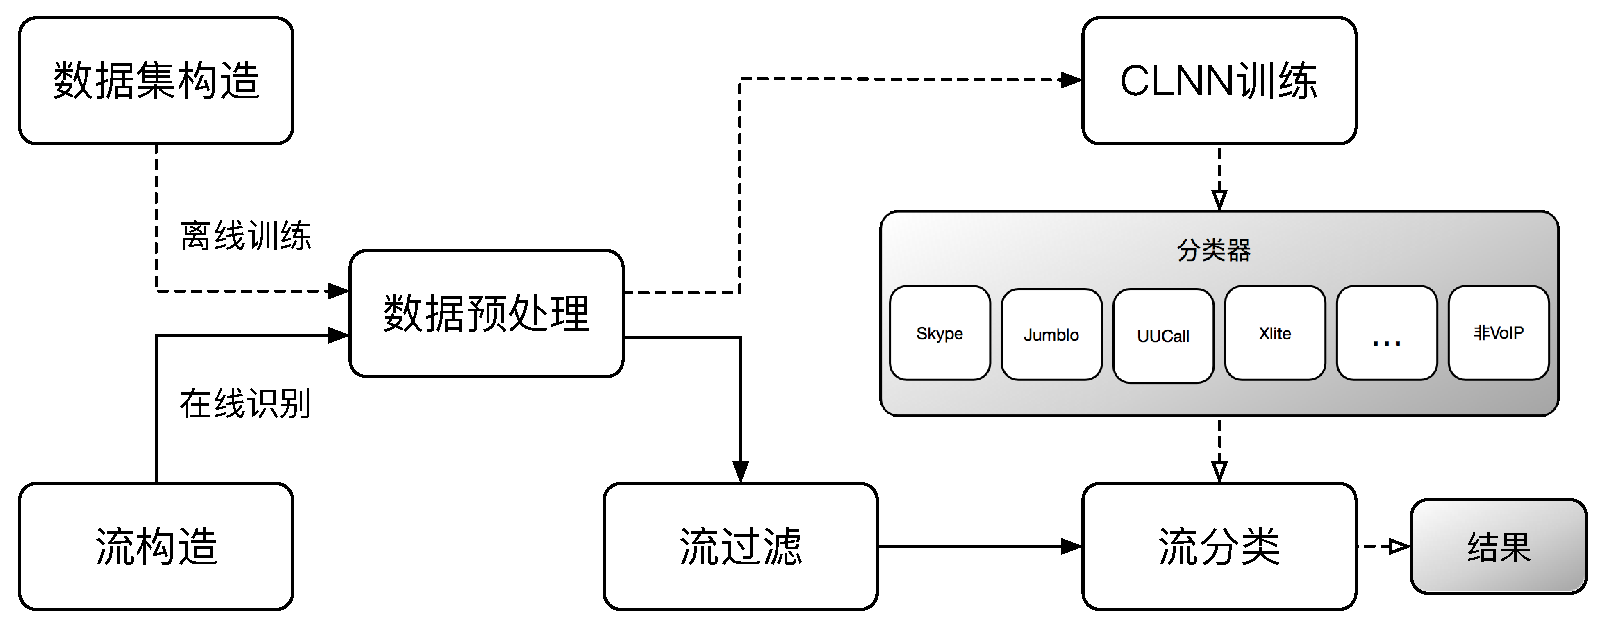
\includegraphics[height=2.5in]{./figures/architecture.eps}
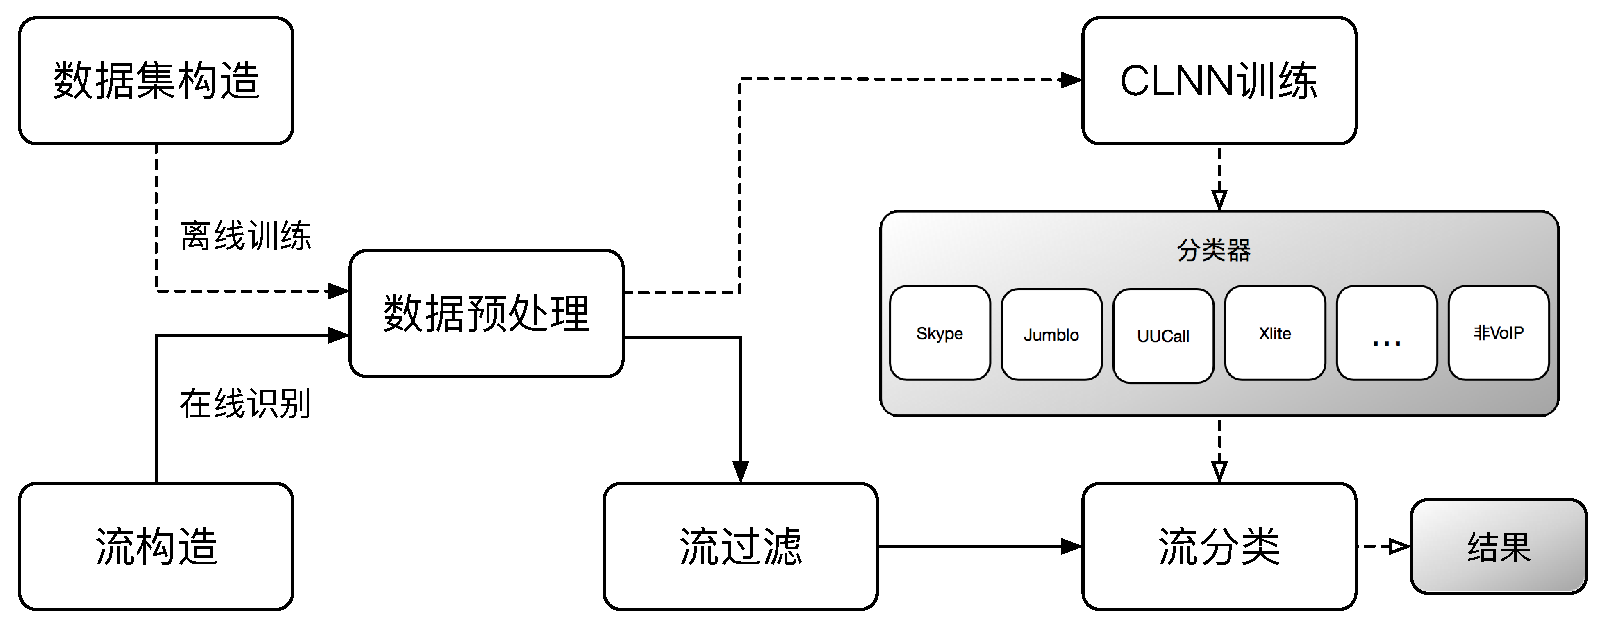
\includegraphics[width=0.9\textwidth]{figures/architecture.eps}
\caption{VoIP流量实时识别框架}
\label{fig:architecture}
\end{figure}

\subsection{离线训练阶段}
离线训练阶段包括数据集的构造、数据预处理、CLNN模型训练和SVM训练等四个过程,其目的是通过深度学习提取VoIP子流的特征集用于训练适于实时识别的分类器。上文我们提到,构造数据集的过程是会将我们采集的原始数据按照应用类型进行标记并且将VoIP完整流按照不同的k值进行分流以适用于实时识别;之后,预处理过程会对数据集及其所对的标签进行预处理工作,数据集中的VoIP子流将会被处理成可输入CLNN模型的矩阵,其对应的标签将会被作为目标矩阵一同输入到CLNN模型进行训练;CLNN模型接收数据集执行训练过程,经过不断的迭代过程,得到具有最小损失的模型,通过该模型提取出的特征集将会用于SVM训练分类器;使用SVM训练所得的分类器的准确率没有CLNN模型高,但是其具有更良好的实时性。如图\ref{fig:architecture}中所示,分类器可以识别出各类型的VoIP应用流量,同时也可对非VoIP的媒体传输流进行识别。

\subsection{在线识别阶段}
在线识别阶段包括流构造、数据预处理、流过滤和流分类几个过程。章节\ref{sec:onlineidentification}中我们提到的3个用于实时识别的组件分别用于执行流构造、流过滤和流分类几个过程。图片\ref{fig:online_3_component}展示了流量捕获器、VoIP流过滤器和分类器工作的基本流程。其中待识别子流中键值为key\_3的子流由于数据包数量达到了k,它将会被送往VoIP流过滤器执行过滤操作。通过过滤器后将会由分类器作出识别结果存入数据库。图中展示了两个被流量捕获器捕获的数据包其键值分别为key\_1和key\_2,由于key\_2数据包未在数据库中查到其对应的识别结果,它将会被用于构造待识别子流等待识别。而key\_1数据包在数据库中查到其识别结果为Skype,该数据包会被判断为Skype数据包。

\begin{figure}[htp]
\begin{center}
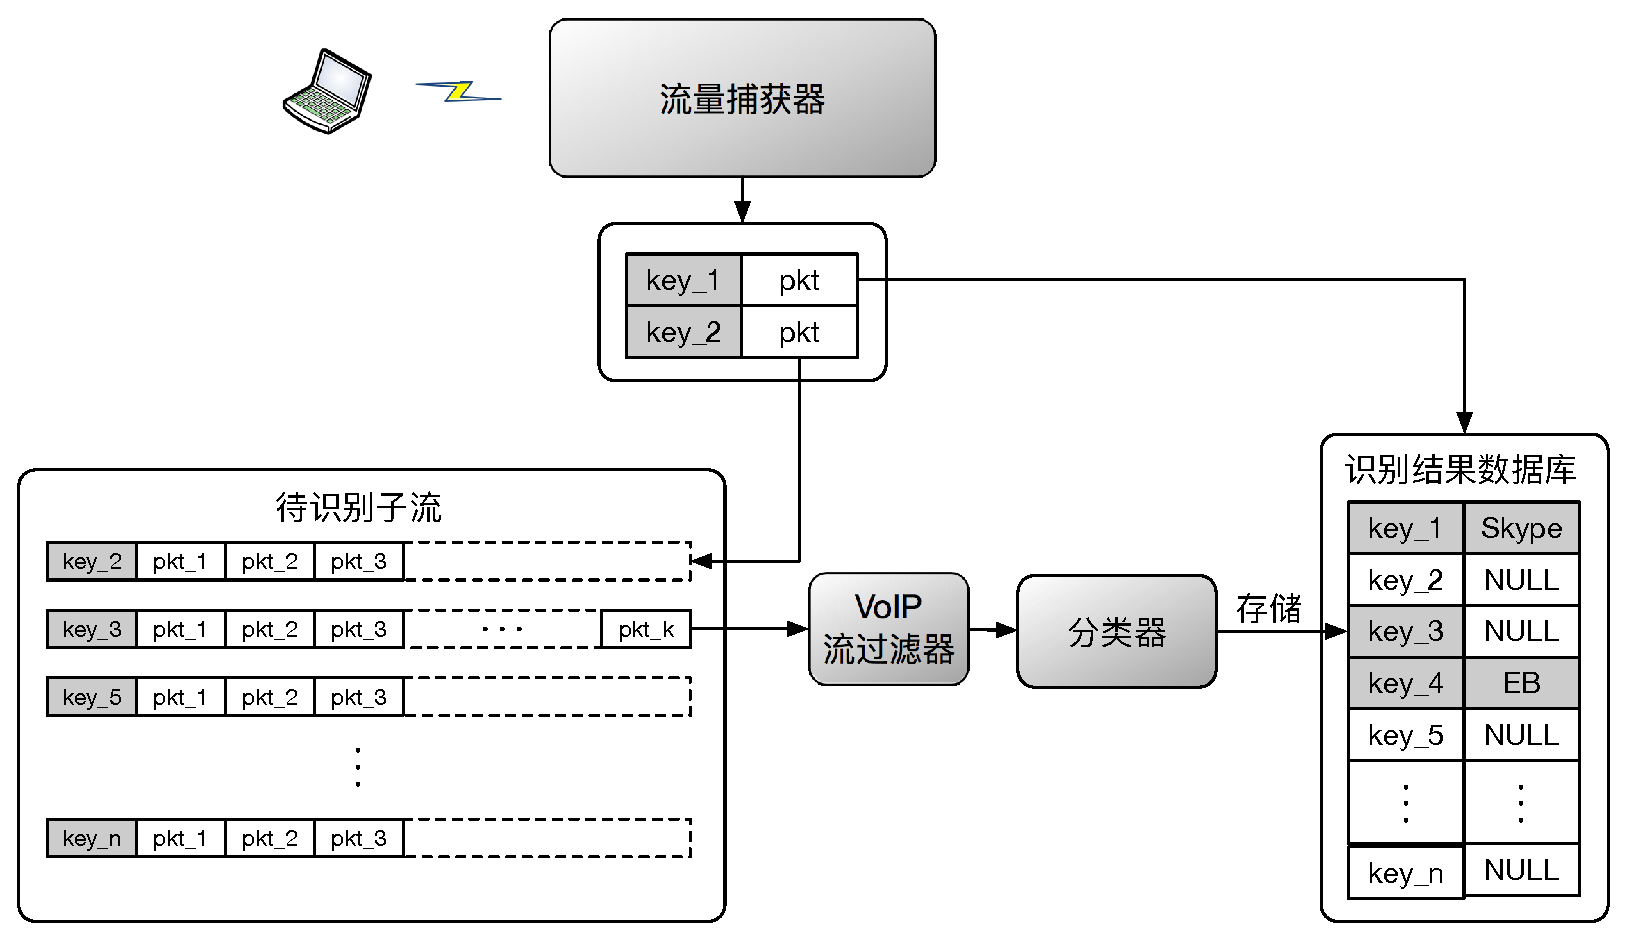
\includegraphics[width=0.9\textwidth]{figures/online_3_component.eps}
\caption{流量捕获器、VoIP流过滤器和分类器工作流程示意图}\label{fig:online_3_component}
\end{center}
\end{figure}

\section{数据集构造}
深度学习是在海量数据的环境中提取有价值的信息,足够海量的数据是深度学习的基础。构造带标签的数据集对于研究人员来说是一项繁重的任务,另外由于VoIP流量的隐私性,国内外没有公开的海量数据集供我们使用。本文所涉及的落地应用主要针对于可以直拨PSTN的VoIP应用,因此采集了10种流行的VoIP应用流量和其他非VoIP流量用于训练深度学习模型。

\subsection{原始数据收集}
为了保证所捕获的VoIP原始流量的多样性,避免因流量过于单一造成所提取的特征集不具备足够的泛化能力,本文使用多台计算机在多种操作系统下进行流量的收集工作,并使用基于线程的流量捕获工具进行流量标记工作。


为了获得较为纯净的数据集,本文在原始数据收集阶段使用基于线程的方法进行捕获工作。在Windows操作系统下,我们使用QPA进行流量捕获。QPA是一款开源的抓包、提供正则表达式识别引擎、按流量类型自动归类、能实时快速的分析软件,我们主要使用其基于进程的工作方式进行流量采集工作。由于QPA未在Linux环境下提供相应软件,我们使用tcpdump工具执行流量捕获工作。当VoIP应用开始通话后,我们首先分析其使用的端口号,针对该端口号使用命令“tcpdump -i eth\_name trans\_protocol port port\_id”进行流量捕获。基于线程和端口的方法使得所捕获的流量可以很容易的按照应用类型进行标记用于深度学习。来自视频应用和游戏的流量都将被标记为非VoIP流量。


\subsection{数据预处理}
捕获的原始数据是以pcap文件的格式存储的,每个pcap文件存储的内容为一次VoIP通话所生成的流量。数据预处理就是要将原始pcap文件处理成可供CLNN模型学习的训练数据,一是要按照章节\ref{sec:construct}中介绍的方法进行子流的划分用于提取适于实时识别的特征集,二是要将子流处理成可输入CLNN模型的矩阵格式。

为了采取多个数据集适应不同程度的实时识别,本文按照k值的不同训练了多个CLNN模型。k值包括2,4,6,8,10,20,40和100,以上多个k值所训练出的模型具有不同程度的实时性。其识别准确率与k值成正比,实时性与k值成反比。图片\ref{fig:datasetprocessing}展示了以pcap文件作为输入预处理后以子流作为输出的过程。输出的子流以文本文件的方式进行保存。

\begin{figure}[htp]
\begin{center}
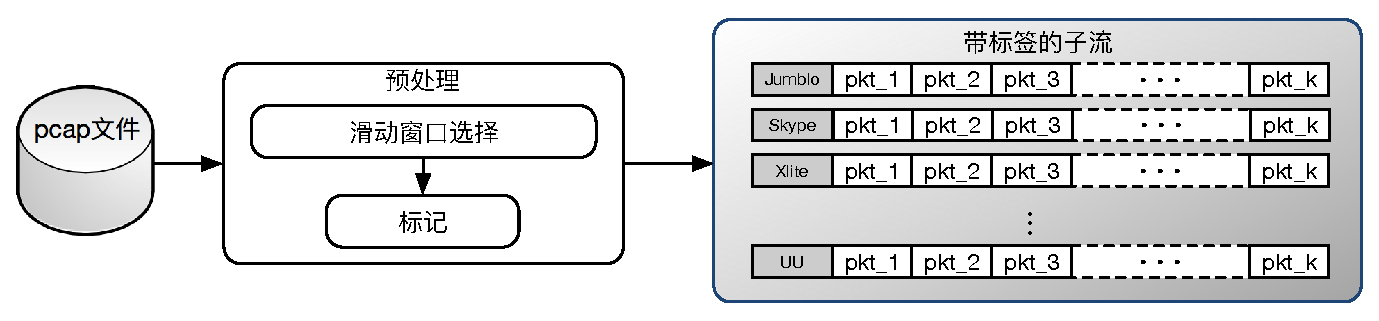
\includegraphics[width=0.9\textwidth]{figures/datasetprocessing.eps}
\caption{数据预处理详情}\label{fig:datasetprocessing}
\end{center}
\end{figure}



按照我们所提出的将VoIP子流转化成矩阵的方法,图片\ref{fig:skype1}展示了一个用于训练的Skype子流$^{100}$图片格式的表现形式。

\begin{figure}[htp]
\begin{center}
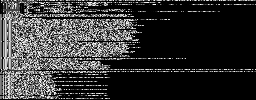
\includegraphics[width=0.8\textwidth]{figures/skype1.png}
\caption{Skype子流$^{100}$的图片表现形式}\label{fig:skype1}
\end{center}
\end{figure}

\section{CLNN模型离线训练}
基于CLNN模型的离线训练过程是进行VoIP流量识别的核心。训练过程中,CLNN模型可以通过对训练数据的学习,将低维层次的特征转化成高维层次的特征,从而构造出用于VoIP流量识别的特征集。CLNN模型通过训练数据集自学习过程中,会在正向传播的过程中计算损失,并通过随机梯度下降的方式逐层向前反馈进行反向传播,从而最小化损失。

本文使用Keras库搭建CLNN模型,Keras是一个基于Theano和TensorFlow的深度学习库,其具有高度模块化和可扩充的特性,并且可以支持CPU和GPU的无缝切换。Keras高度的支持CNN和RNN的结合,本文使用的CNN和LSTM的策略可以很简单的使用Keras实现。Keras提供的函数式模型是用户定义多输出模型、非循环有向模型或具有共享层的模型等复杂模型的途径,本文使用函数式模型进行了CNN和LSTM的结合,从而创建了具备更强的提取VoIP流量特征能力的模型。

CLNN模型经过不断的迭代学习后,输出结果就是用于VoIP子流识别的一系列权重值。CLNN模型使用这些权重值进行正向计算从而可以计算出VoIP子流的识别结果。

\subsection{模型基本结构}
CLNN模型在学习过程中会生成大量的参数,大量的参数也是CLNN模型准确识别的基础。本节将以k=100对CLNN模型每层所使用的具体参数进行详细介绍。之后列出本文训练的8种模型生成的权值参数个数以及保存权值的HDF5文件大小。

\newcommand{\tabincell}[2]{\begin{tabular}{@{}#1@{}}#2\end{tabular}}
\begin{table} [htb]
  \caption{CLNN模型参数详情}
  \label{tab:clnnparams}
  \centering
\begin{tabular}{|c|c|c|c|}
\hline
\multicolumn{3}{|c|}{\textbf{$CNN+Dense$}} & \textbf{LSTM}\\
\hline

\multirow{3}{*}{Conv1}&
 输入& $100 \times 256 \times 1$ & \multirow{21}{*}{\tabincell{c}{输入:$100 \times 256$\\单元:$100$\\权值个数:$142800$\\Dropout:$0.5$}}\\ 
\cline{2-3}
  & 参数 & 卷积核:$5 \times 5 \times 48$;步长:$2$ &  \\
\cline{2-3}
  & 输出 & 权值个数:$1248$;Dropout:$0.5$ &  \\  

\cline{1-3}
\multirow{3}{*}{Conv2}&
输入& $50 \times 128 \times 48$ & \\
\cline{2-3}
  & 参数&卷积核:$3 \times 3 \times 128$;步长:$2$  &  \\
\cline{2-3}
  & 输出 & 权值个数:$55424$;Dropout:$0.5$ &  \\  

\cline{1-3}
\multirow{3}{*}{Conv3}&
输入& $25 \times 64 \times 128$ & \\
\cline{2-3}
  & 参数&卷积核:$3 \times 3 \times 192$;步长:$1$&  \\
\cline{2-3}
  & 输出 & 权值个数:$221376$;Dropout:$0.5$ &  \\  

\cline{1-3}
\multirow{3}{*}{Conv4}&
输入& $25 \times 64 \times 192$ & \\
\cline{2-3}
  & 参数&卷积核:$3 \times 3 \times 192$;步长:$1$ &  \\
\cline{2-3}
  & 输出 & 权值个数:$331968$;Dropout:$0.5$ &  \\  

\cline{1-3}
\multirow{3}{*}{Conv5}&
输入& $25 \times 64 \times 192$ & \\
\cline{2-3}
  & 参数&卷积核:$3 \times 3 \times 128$;步长:$1$ &  \\
\cline{2-3}
  & 输出 & 权值个数:$221312$;Dropout:$0.5$ &  \\  

\cline{1-3}
\multirow{3}{*}{Dense1}&
输入& 204800 & \\
\cline{2-3}
  & 参数&单元:$2048$ &  \\
\cline{2-3}
  & 输出 & 权值个数:$419432448$;Dropout:$0.5$ &  \\  

\cline{1-3}
\multirow{3}{*}{Dense2}&
输入& 2048 & \\
\cline{2-3}
  & 参数&单元:$100$ &  \\
\cline{2-3}
  & 输出 & 权值个数:$204900$;Dropout:$0.5$ &  \\  
\hline
\multirow{3}{*}{Dense3}&
输入&\multicolumn{2}{c|}{$200$} \\
\cline{2-4}&
参数&\multicolumn{2}{c|}{单元:$11$}\\
\cline{2-4}&
输出&\multicolumn{2}{c|}{权值个数:$2211$}\\
\hline
\end{tabular}
\end{table}

表格\ref{tab:clnnparams}展示了CLNN模型每层所采用的参数详情。表格所示由两部分组成,第一部分是由CNN和Dense组成的用于提取频域特征的模型,第二部分是LSTM层用于提取时域特征。两部分在Dense3也就最后一个全连接层进行组合,Dense3将频域特征和时域特征进行组合最大患的提取VoIP流量携带的特征。以第一层Conv举例,输入为$100 \times 256 \times 1$的矩阵,卷积核大小为$5 \times 5 $,深度为48。通过${W} = (r_{filter} \times c_{filter} \times d_{input} + b) \times d_{filter}$可以计算该层权值个数为1248,其中每个神经元包含$5 \times 5 \times 1$权值和一个偏差。以第一层Dense层举例,输入为204800维的向量,输出为2048维的向量,通过${W} = (dim_{input} + b) \times dim_{output}$可以计算其权值个数为419432448。LSTM层输入为$100 \times 256$的矩阵,输出单元为100,可以通过${W} = 4 \times (dim_{output}+r_{input}+1)\times dim_{output}$计算其权值个数,其中4代表每个LSTM单元包括4个激活函数。



\subsection{Keras搭建模型}
本文使用Keras提供的Model类搭建函数式模型,需要导入Keras提供的models包。使用
\begin{center}
model=Model(input=subflows,output=[model])
\end{center}
创建模型。之后,向该模型中添加隐层,本文主要使用了3种隐层,卷积层、全连接层和LSTM层。依次可以使用
\begin{center}
model = Conv2D(filters, kernel\_size, strides, activation)(model)
\end{center}
\begin{center}
model = Dense(units, activation)(model)
\end{center}
\begin{center}
model = LSTM(units, activation)(model)
\end{center}
添加到CLNN模型中。另外,本文选择性使用了池化层(MaxPooling2D)和失活层(Dropout)加速训练的过程。在维度转换时,本文使用了平滑层(Flatten)和变形层(Reshape)提供的支持。

本文搭建的CLNN模型最主要的特性是针对频域特征和时域特征同时进行提取,最后使用全连接层综合两个类型的特征。以下代码段展示了如何将CNN和LSTM提取的特征进行组合。
\begin{lstlisting}[language={Python},label={lst:concat}]  
input = Input(input_shape)
conv = create_cnn_layers(input)
lstm = create_lstm_layers(input, input_shape[0])
model = concatenate([conv, lstm],axis=1)
model = Dense(nb_class, activation='softmax')(model)
\end{lstlisting}  

\subsection{迭代训练}
CLNN模型迭代训练是通过训练数据集不断调整权值寻找具有最小误差的权值的过程。

本文使用随机梯度下降的算法进行权值的更新,同时在随机梯度下降时引入冲量,冲量用于表示上一梯度对当前梯度的贡献率。梯度下降算法采用小批量更新的策略,每一批样本数据计算一次损失函数并更新参数。随机梯度下降优化器可通过SGD类进行定义。
\begin{center}
sgd = SGD(lr=0.0, decay=0.0, momentum=0.9, nesterov=True)
\end{center}
为CLNN模型配置损失函数和优化器类型通过compile函数完成,
\begin{center}
model.compile(loss='categorical\_crossentropy', optimizer=sgd)
\end{center}
以上配置所使用的损失函数为针对多类的对数损失函数。

上文中定义随机梯度下降函数时没有为SGD指定学习率,因为本文采取每轮训练完成后都要对学习率进行更新的策略。以下代码段为对上一章中介绍的公式\ref{equ:decay}的具体实现。
\begin{lstlisting}[language={Python},label={lst:decay}]  
def step_decay(epoch):
    initial_lrate = 0.01
    drop = 0.5
    epochs_drop = 5.0
    lrate = initial_lrate * 
        math.pow(drop,math.floor((1+epoch)/epochs_drop))
    print(lrate)
    return lrate
lrate = LearningRateScheduler(step_decay)
\end{lstlisting}  

训练中使用EarlyStopping优化训练行为,当损失不再减小时则提前停止训练过程。
\begin{center}
earlystopping = EarlyStopping(monitor='val\_loss', patience=1)
\end{center}

我们在训练中对全部数据指定进行20轮的计算,当然,在满足EarlyStopping的条件后训练也会提前结束。每200个样本计算后反向传播进行梯度的更新。以下函数最后的callbacks参数展示对学习率更新以及EarlyStopping的调用。
\begin{center}
model.fit(X\_train, Y\_train, batch\_size=200,validation\_data=(X\_val, Y\_val),epochs=20,callbacks=[early\_stopping,lrate])
\end{center}


\subsection{模型保存}
经过训练得到的最终模型需要进行存储,模型分为两个部分进行存储。一是需要对CLNN模型的基础架构进行存储,我们使用json格式的文件进行存储;二是要对训练后的模型的权重参数进行保存,我们使用可提供层次数据格式存储的HDF5进行存储。在实时识别阶段我们将使用该模型进行VoIP流量的识别。表格\ref{tab:params}展示了本文训练所得的8个CLNN模型生成的权值个数及存储为HDF5文件得大小详情。

\begin{table}
  \caption{8个CLNN模型生成的权值个数及HDF5文件大小详情}
  \label{tab:params}
  \centering
  \begin{tabular}{l l l l}
    \hline
    \textbf{CLNN-k} & \textbf{输入} & \textbf{权值个数}&\textbf{HDF5(MB)}\\
    \hline
    k=2      & ${2 \times 256 \times 1}$  & 17,818,697  &87  \\
    k=4      & ${4 \times 256 \times 1}$  & 17,820,823  &87  \\
    k=6      & ${6 \times 256 \times 1}$  & 34,600,197  &154  \\
    k=8      & ${8 \times 256 \times 1}$  & 34,602,387  &154 \\
    k=10     & ${10 \times 256 \times 1}$  & 51,381,825  &221.6  \\
    k=20     & ${20 \times 256 \times 1}$  & 84,947,847  &355.8 \\
    k=40     & ${40 \times 256 \times 1}$  & 168,859,507  &691.3  \\
    k=100    & ${100 \times 256 \times 1}$  & 420,613,687  &1619.3  \\
    \hline
  \end{tabular}
  %\caption{The details of Alexnet parameters.}
\end{table}

\section{VoIP流量实时识别系统}
VoIP流量实时识别系统是部署在大规模真实网络出入口节点上的用于在线识别VoIP流量的分布式系统。为了应对大规模真实网络上复杂多变的环境,我们采用Apache Kafka流处理平台接入真实网络环境。Kafka流处理平台使用ZooKeeper作为其后端分布式服务器管理、协调Kafka代理,可以为处理实时数据提供高吞吐、低延迟的性能,解决了真实网络中流速不均衡造成的难题。其次,Kafka除了为我们提供负载均衡的环境之外,也作为我们的数据备份模块备份网络流量。为了达到实时计算的目的,我们采用Apache Storm作为流式计算框架执行计算任务。用户通过自定义Spout和Bolt指定信息源和计算措施从而达到批量、分布式处理流式数据的目的。本节我们将分为Kafka和Storm两个模块进行介绍。

\subsection{Kafka模块}
Kafka模块是用于直接对接真实网络环境的基础模块,其可以按照不同交换机和路由器创建标题,供Storm模块进行消费。

图片\ref{fig:kafka}展示了真实网络如何接入Kafka集群的结构图。本文实验中将局域网中的路由器接入Kafka集群模仿真实网络环境中的交换机。

\begin{figure}[htp]
\begin{center}
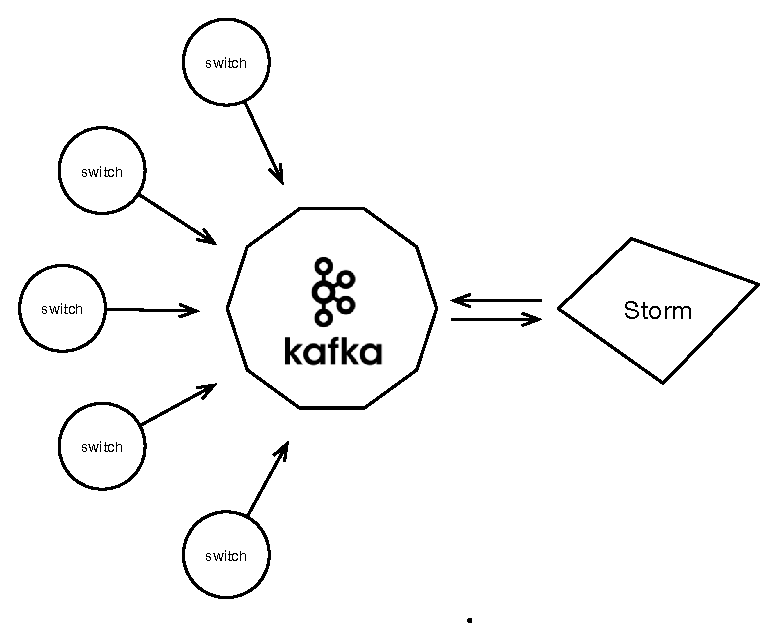
\includegraphics[width=0.7\textwidth]{figures/kafka.eps}
\caption{真实网络环境接入Kafka集群结构图}\label{fig:kafka}
\end{center}
\end{figure}

Kafka提供良好的Java编程接口,我们主要使用其提供的生产者接口将真实网络中的流量发送到Kafka集群中。以下分别为发送单条数据和发送多条数据所对应的接口。

\begin{center}
public void send(KeyedMessage<K,V> message) 
\end{center}

\begin{center}
public void send(List< KeyedMessage<K,V> > messages) 
\end{center}

\subsection{Storm模块}
Storm模块是支持实时识别的核心模块,其对来自Kafka集群的动态的、连续的以及大数据量的流量作出及时的处理。

本文使用Kafka Spout作为消费者客户端消费Kafka集群中未处理的流量,同时Kafka Spout也作为Storm拓扑结构的数据源将流量吐到Storm拓扑中进行处理。其次,我们使用两个Bolt分别作为流量捕获器的UDP识别和分流部分,后继Bolt可能是一个VoIP流过滤器也可能直接是一个分类器,这根据不同的k值作出不同调整。具有较小k值的VoIP流不易进行初步VoIP流过滤操作,其次较小的k本身要求要高的实时性,因此不经过VoIP流过滤器直接送入分类器进行识别。最后一个Bolt提供写入Redis数据库的操作。图片\ref{fig:storm}展示了Storm模块的拓扑结构图。其中分类器Bolt对应多种CLNN模型所构成的分类器,它们产生的结果和该结果所对应的可能性都将输出到Redis数据库中,网络管理员可以根据实时性和准确度要求拿取符合要求的结果。

\begin{figure}[htp]
\begin{center}
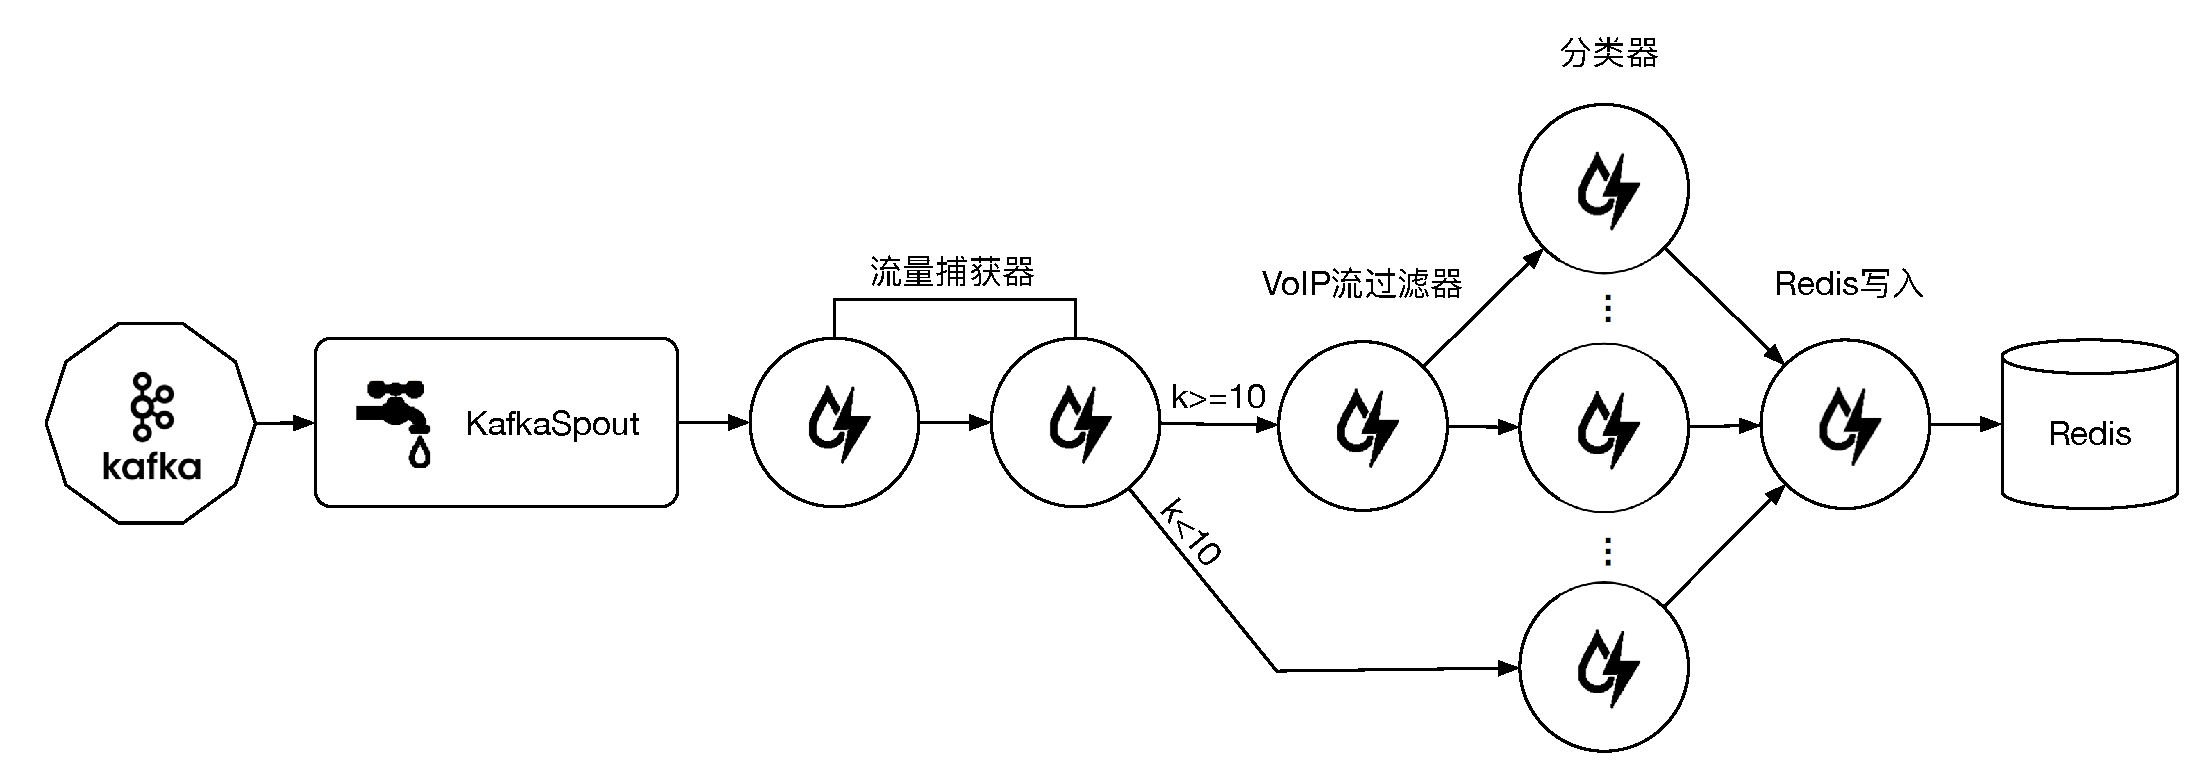
\includegraphics[width=0.9\textwidth]{figures/storm.eps}
\caption{Storm模块拓扑结构图}\label{fig:storm}
\end{center}
\end{figure}
以下代码段展示了Storm拓扑的搭建过程。
\begin{lstlisting}[language={Java},label={lst:storm}]  
TopologyBuilder tb = new TopologyBuilder();
tb.setSpout("spout", new TrafficSpout(), 3);  // executor num
tb.setBolt("udpbolt", new UDPBolt()).shuffleGrouping("spout");
tb.setBolt("pendingflowsbolt", new PendingFlowsBolt())
        .fieldsGrouping("udpbolt", new Fields("key"));
tb.setBolt("classifierbolt10", new ClassifierBolt10())
        .shuffleGrouping("pendingflowsbolt", "10");
tb.setBolt("filterbolt", new FilterBolt())
        .shuffleGrouping("pendingflowsbolt", "100");
tb.setBolt("classifierbolt100", new ClassifierBolt())
        .shuffleGrouping("filterbolt");
tb.setBolt("rediswriterbolt", new RedisWriterBolt())
        .shuffleGrouping("classifierbolt10")
            .shuffleGrouping("classifierbolt100");
\end{lstlisting}  

\section{本章小结}
本章依托第三章设计的移动应用流量识别算法,实现了一个移动应用流量识别系统。本章第一节首先系统的介绍整体框架,分为离线训练阶段和在线识别阶段做了简单介绍;第二节对本文采用的构建数据集的方法和数据集详细信息做了介绍;第三节对本文所使用的CLNN模型的结构做了详细介绍,并从编程的角度介绍了模型的搭建、训练和输出的过程;最后第四节介绍了为支撑大规模网络环境中的识别,我们采用的Kafka和Storm框架,并使用这两种框架开发了适用于本文所提出的方法的应用环境。



\chapter{实验结果和性能评估}
本章将从CLNN模型准确率和VoIP识别系统的实时性两个方面进行评估。针对本文所采取的VoIP流量,使用本文所搭建的CLNN模型进行训练和验证,并分析了8个不同k值训练出的CLNN模型的识别准确率。同时,为证明本文所提取的特征集的有效性,我们使用4种机器学习的方法通过该特征集训练数据集并进行了对比。最后,从实时性的角度分析实时系统的可用性。

\section{实验基础}
\subsection{实验环境}
实验环境包括开发环境和运行环境两个部分,开发环境用于训练CLNN模型和实时系统开发,运行环境用于搭建分布式服务器、运行Kakfa和Storm集群、存储识别结果和回放VoIP流量。

表格\ref{tab:dev}展示了本文开发环境和软件。本文深度学习方面的内容基于Python开发,使用的深度学习框架为Keras。本文使用GPU环境加速深度学习过程,使用CUDA作为其运算平台。分布式集群相关使用Java进行开发。
\begin{table} [htb]
\caption{开发环境}\label{tab:dev}
\small
\centering
%[t]
{
\begin{tabular}{ccl}
  \toprule
          &   项目 &   具体环境及版本\\
  \midrule
       \multirow{3}{*}{硬件环境}  & CPU &   四核 3.6GHz Intel Core i7 \\
                 &    GPU    &  NVIDIA GeForce GTX 1070  \\
                 &    RAM    &  8GB  \\ 
  \midrule
       \multirow{4}{*}{软件环境} & 操作系统 & CentOS7  \\ 
                 & GPU运算平台 & CUDA Toolkit 8.0\\
                 &    深度框架 & Keras \\
                 &   编程语言 & Python 2.7.10, Java 1.8.0\\
 \bottomrule
\end{tabular}
}
\end{table}

表格\ref{tab:runtime}展示了本文VoIP实时识别系统的运行环境。本文使用ZooKeeper提供分布式协调服务,Kafka和Storm作为运行在ZooKeeper之上的分布式应用提供存储和计算功能。键值数据库使用Redis提供分布式查询功能。本文为模拟真实网络环境的VoIP流量,使用了tcpreplay软件回放我们采集到的VoIP流量。
\begin{table} [htb]
\caption{运行环境}\label{tab:runtime}
\small
\centering
%[t]
{
\begin{tabular}{ccl}
  \toprule
          &   项目 &   具体环境及版本\\
  \midrule
       \multirow{1}{*}{硬件环境}  & 服务器 &  3台, RAM 8GB, 磁盘空间 200GB  \\
  \midrule
       \multirow{5}{*}{软件环境} & 操作系统 & CentOS7  \\ 
                 &    分布式系统 & ZooKeeper 3.4.12 \\
                 & 集群服务 &Kafka 2.0.0, Storm 1.2.2\\
                 &    数据库 & Redis 5.0.3 \\
                 &   回放软件 & tcpreplay\\
 \bottomrule
\end{tabular}
}
\end{table}


\subsection{数据集}
本文针对10种流行的VoIP应用和多种非VoIP的视频和即使游戏应用进行了流量的捕获工作。为了提升识别的泛化能力,我们部署了8台计算机,其中6台计算机安装了Windows操作系统,2台计算机安装了Linux操作系统,2台Linux计算机安装了提供支持在Linux环境下使用的4种VoIP应用,6台装载Windows操作系统的计算机均安装了10种VoIP应用。其次我们捕获了视频应用、视频通话应用和即时游戏应用的UDP流量作为非VoIP应用流量。为了保证VoIP通话线路的泛化性,我们从国内包括河北省、吉林省、广东省和四川省多个地方拨打电话用于流量获取工作。

本文将采集到的数据分成两个数据集,数据集1用于训练CLNN模型,数据集2用作回放流量验证实时系统的性能。\ref{tab:traffic}展示了数据集1的统计信息和经过处理后用于训练的子流$^{10}$个数。数据集2不做子流处理,其流量大小与数据集1相同,将通过tcpreplay软件进行流量回放验证实时系统的识别效率、准确率和鲁棒性。训练过程中数据集1中的80\%子流用作训练CLNN模型,20\%的子流用于训练过程中验证准确率。

\begin{table}[htbp]
  \caption{数据集1详细信息}
  \label{tab:traffic}
  \centering
  \begin{tabular}{l l l l}
    \hline
    \textbf{VoIP应用类型} & \textbf{平台} & \textbf{数据集大小(MB)}& \textbf{子流数(k=10)}\\
    \hline
    Skype      & Windows, Linux  & 3908.8  &  669984  \\
    UUCall      & Windows  & 2709.4  &  691566  \\
    KCCall      & Windows  & 3128.8  &  808224  \\
    ALTCall      & Windows  & 2795.2  &  692002  \\
    Jumblo      & Windows, Linux  & 3704.6  &  871468  \\
    Zoiper      & Windows, Linux  & 4418.1  &  677114  \\
    Xlite      & Windows, Linux  & 5165.3  &  638288  \\
    Eyebeam      & Windows  & 4524.7  &  616773  \\
    ExpressTalk      & Windows  & 4633.1  &  602637  \\
    Bria      & Windows  & 4476.0  &  598724  \\
    non-VoIP      & Windows  & 11324.5  &  973522  \\
    \hline
  \end{tabular}
  %\caption{The details of dataset1.}
\end{table}

\subsection{训练参数}
训练过程中使用的SGD算法是一种学习率非自适应的算法,学习率的设置对实验结果有直接的影响。我们结合深度学习一般经验并按照实验结果进行调整,初始学习率设置为0.01,衰减规则按照本文以上所述每两轮训练进行一次衰减。nesterov动量因子设置为0.9,它会吸收上一梯度90\%的贡献。我们针对8个k值分别对数据集训练了20轮,每200个样本进行一次梯度更新。


\section{CLNN模型评估}
\subsection{评估指标}
在多分类问题中,不同的场景需要不同的评估指标。一般来说,准确率(Accuracy)就可以评估一个分类模型的性能,用于衡量分类正确的比例。可以使用如下公式计算准确率:
\begin{equation}
Accuracy = \frac{1}{n} \sum\limits_{i = 1}^n {1_{\hat{y_i}={y_i}}}
\end{equation}
其中,$\hat{y_i}$表示被分类模型预测的类别,${y_i}$表示样本的真实类别。准确率是一个适用范围最广的评估指标,可以反映系统的全局识别性能,但是准确率在反映分类器对正负样本的识别能力上有着不足。本文引入真正类率(True Positive Rate, TPR)来表达分类器所识别出的正实例占所有正实例的比例,负正类率(False Positive Rate, FPR)在表达能力上与TPR是互补的关系。对于二分类问题,即将样本分为正类和负类两种情况的问题来说,会出现4种分类结果:如果一个实例是正类并且也被预测成正类,即为真正类(True Positive, TP),如果实例是负类被预测成正类,称之为假正类(False Positive, FP)。相应地,如果实例是负类被预测成负类,称之为真负类(True Negative, TN),正类被预测成负类则为假负类(False Negative, FN)。通过这种分类方式,我们重新表达准确率如下:
\begin{equation}
Accuracy = \frac{{TP + TN}}{{TP + TN + FP + FN}} 
\end{equation}
评估指标TPR和FPR计算如下:
\begin{equation}
TPR = \frac{{TP}}{{TP + FN}}
\end{equation}
\begin{equation}
FPR = \frac{{FP}}{{FP + TN}}
\end{equation}
\subsection{识别性能评估}
根据以上CLNN模型架构及实验基础中使用的参数,我们对11类流量分为8个k值进行了训练得到了8个CLNN模型。本节将对这8个模型按照第一节中介绍的评估指标进行评估。

表格\ref{tab:acc4models}展示了8个模型对训练数据集和验证数据集识别的准确率。训练数据集来自数据集1中的80\%,验证数据集来自数据集1中的20\%。我们可以看出在k值越小时,训练所得模型的识别性能越低。当我们使用由2个数据包构成的子流训练模型时,由于子流携带的课识别的特征太少,CLNN模型的识别准确率仅仅达到65\%;对由4个数据包组成的子流进行识别时,准确率提高到了87\%。当数据包个数达到6个时,识别准确率已经达到了98\%。如表中所示,当k值个数达到10时,k值再增加对识别率的提高作用很小,反而会降低系统的实时性。因此,在我们的实时系统中,我们部署了k值从6到100的6个模型,系统管理员将根据事件的紧急程度和所需准确率进行考量作出选择。
\begin{table}
  \caption{8个模型对训练数据集和验证数据集的识别率}
  \label{tab:acc4models}
  \centering
  \begin{tabular}{l l l l}
    \hline
    \textbf{模型k} & \textbf{损失} & \textbf{训练集}&\textbf{验证集}\\
    \hline
    k=2      & 0.795628  & 0.658810  &0.623340  \\
    k=4      & 0.320275  & 0.874460  &0.882680 \\
    k=6      & 0.091234  & 0.987510  &0.982390 \\
    k=8      & 0.034948  & 0.994820  &0.995510 \\
    k=10     & 0.018984  & 0.997720  &0.998350  \\
    k=20     & 0.007481  & 0.998530  &0.998470 \\
    k=40     & 0.014981  & 0.996550  &0.997640  \\
    k=100    & 0.001795  & 0.999630  &0.999710  \\
    \hline
  \end{tabular}
\end{table}

%这里要改,不再使用dataset2作验证
因为训练过程中普遍存在过拟合的现象,甚至在验证阶段可能不会表现出来。因此我们使用数据集2进行全面的验证。图片\ref{fig:fprtpr}中的前十个图表展示了使用数据集2进行验证的10种VoIP应用流量所对应的TPR,后两个图表展示了数据集2的FPR和TPR分布。很明显的,在前4张图表中我们可以看到一些异常值,分别是使用模型-20进行识别Skype流量、模型-4识别Xlite流量、模型-6识别Eyebeam流量和模型-2识别Bria流量时,这表明这四种模型在训练时针对这几种流量出现了过拟合现象。我们在实时识别过程的过程中暂时放弃使用这几个模型识别出的结果对应四种流量的结果。在未来的研究过程中,第一步我们需要将数据集2合并到数据集1中再次训练,第二步我们考虑加入L1和L2正则层避免过拟合现象。抛除以上几个异常值,综合显示CLNN模型有优秀的识别性能。

\begin{figure*}[htp]
\begin{center}
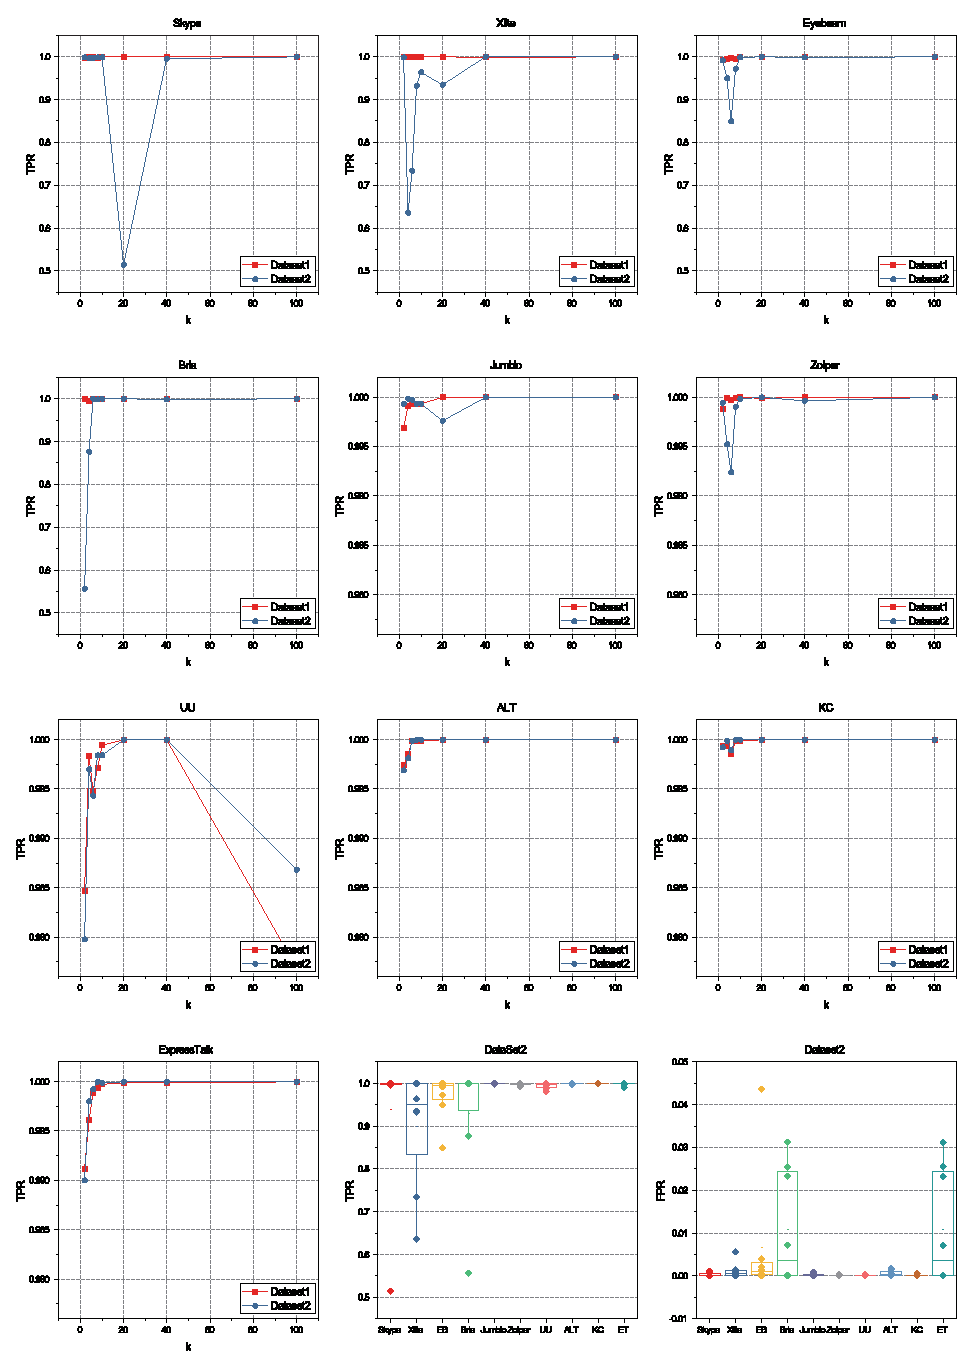
\includegraphics[width=1\textwidth]{figures/fprtpr.eps}
\caption{8种CLNN模型的TPR和FPR结果}\label{fig:fprtpr}
\end{center}
\end{figure*}

图片\ref{fig:tf}展示了针对两个数据集识别时识别正确和识别错误的结果所对应的概率分布。如图所示识别正确的结果所对应的识别概率普遍接近于1,而识别错误的结果所对应的概率分布在0.2-0.98之间,普遍要低于识别正确的结果所对应的概率。该概率将作为实时识别系统初步判断识别结果的阈值。

\begin{figure}[htp]
\begin{center}
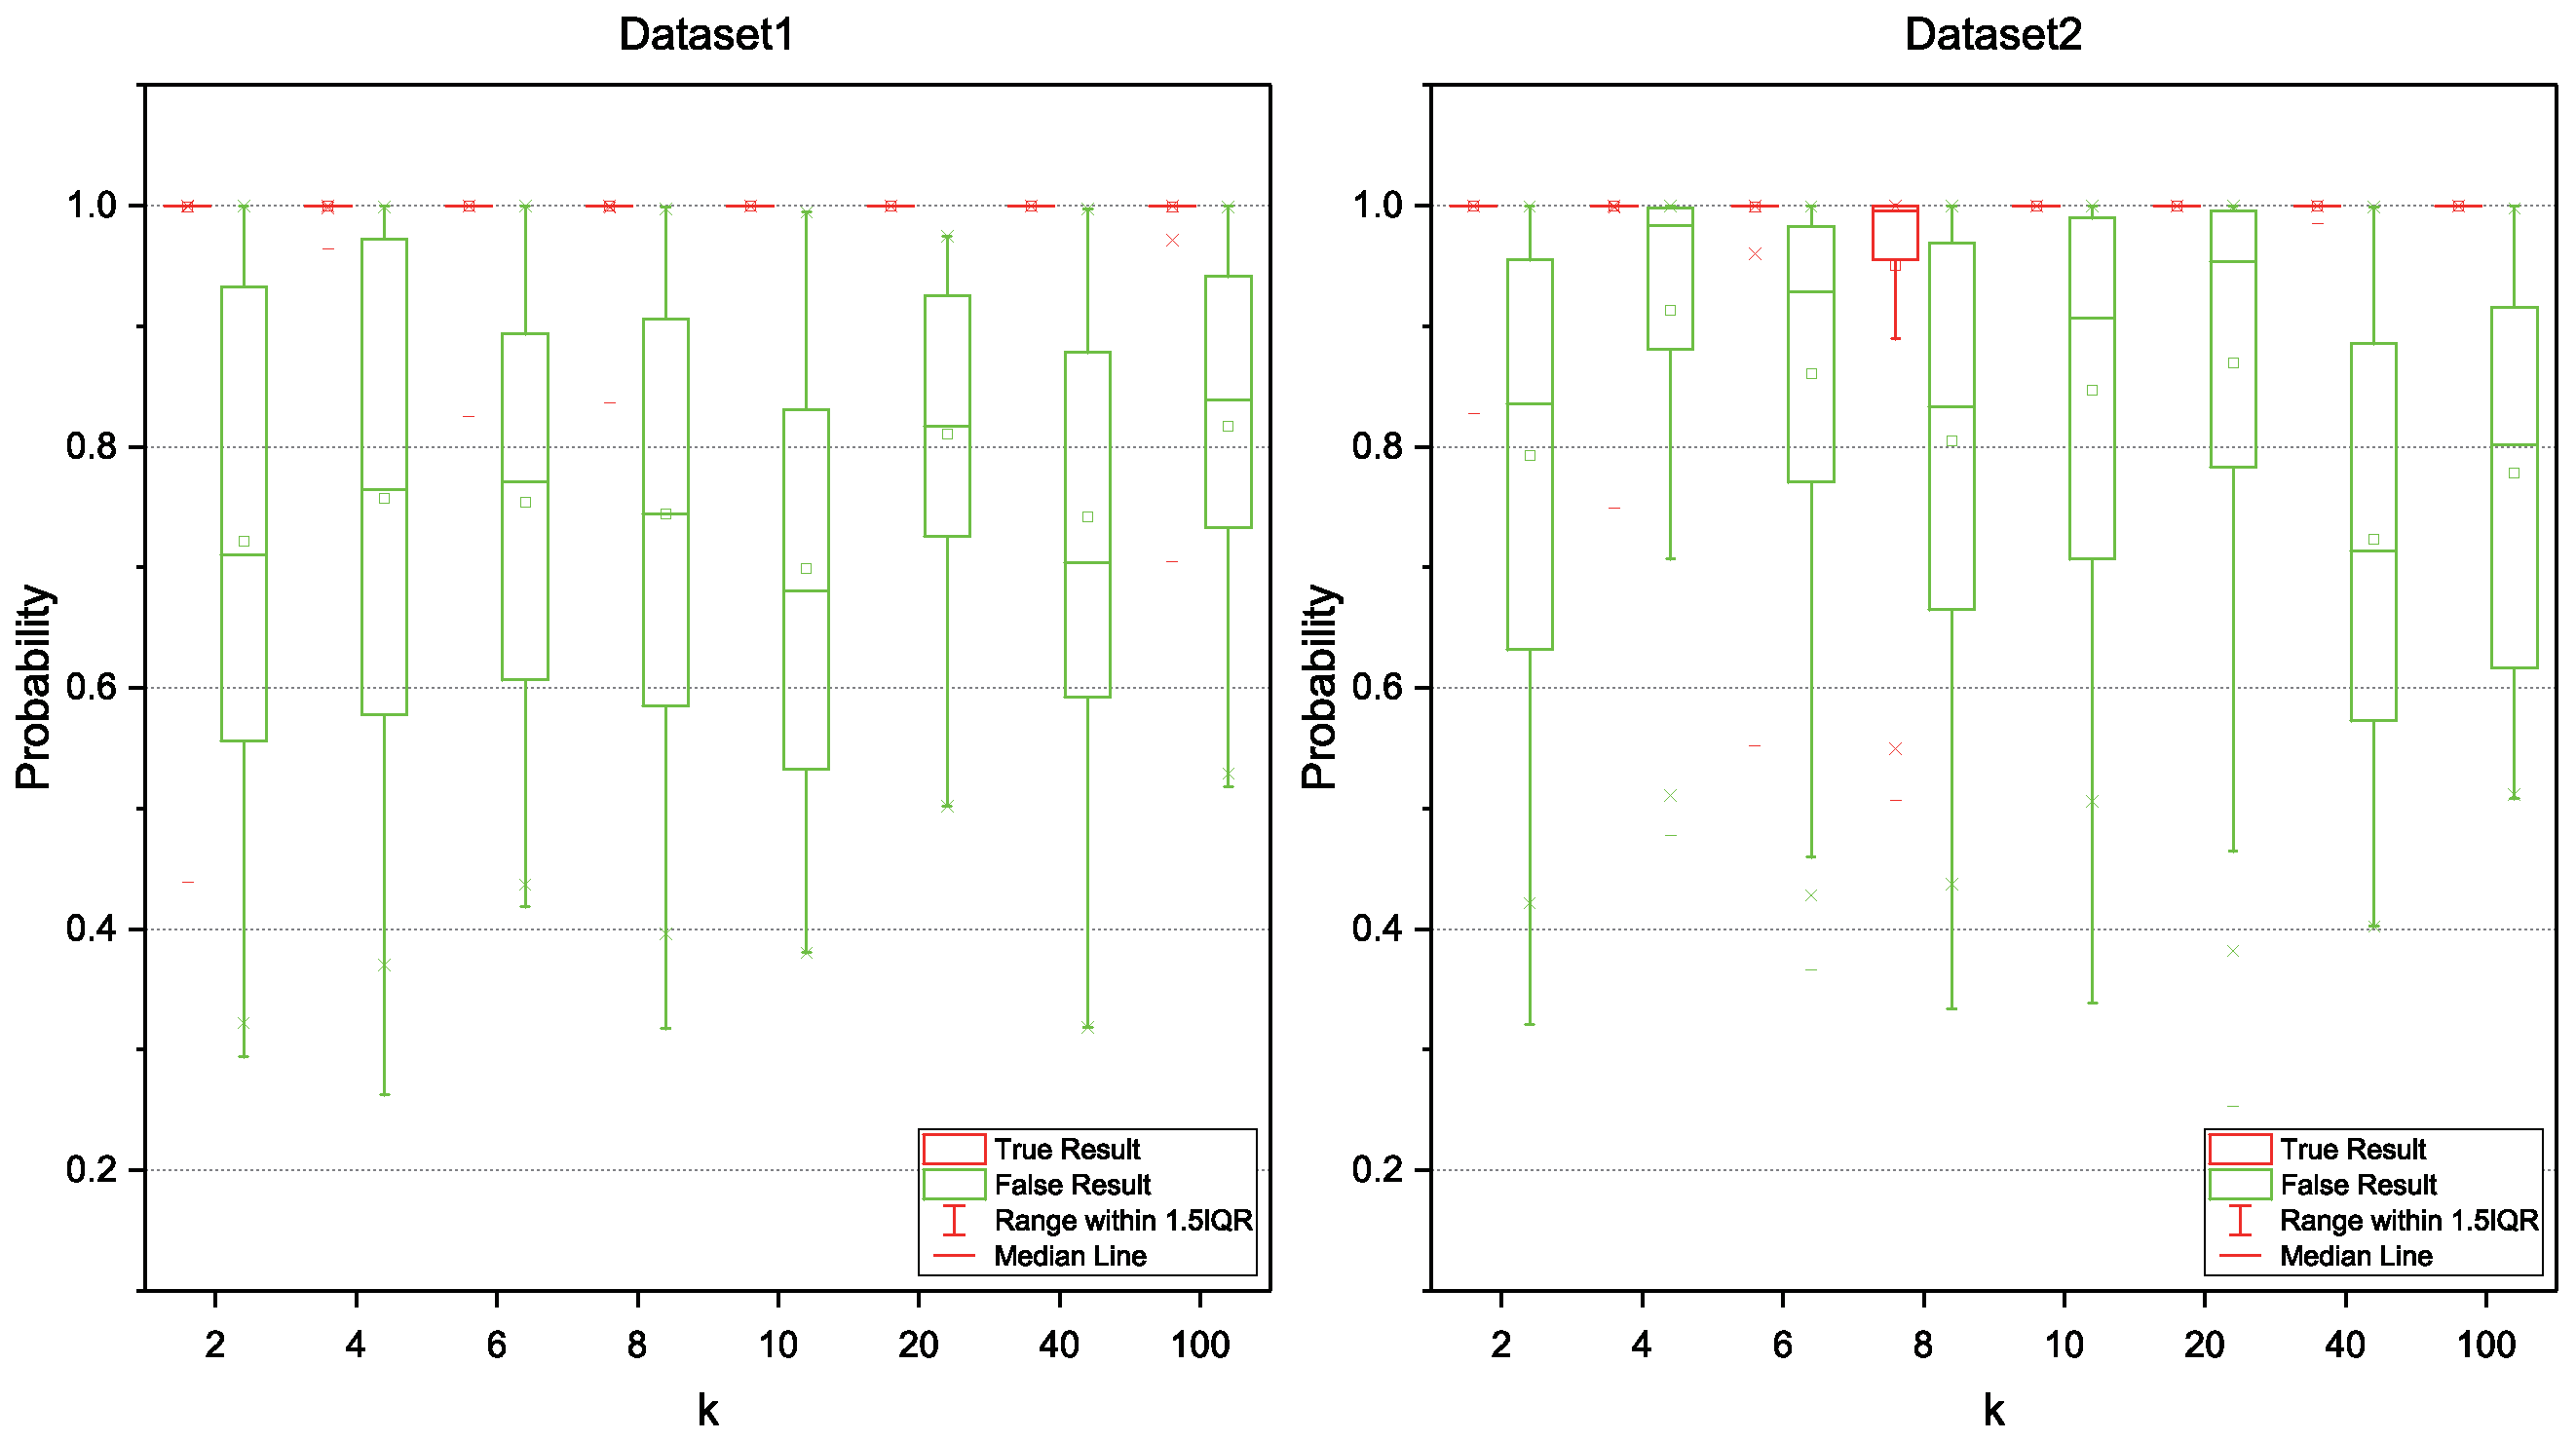
\includegraphics[width=1\textwidth]{figures/tf.eps}
\caption{识别结果的概率分布状况}\label{fig:tf}
\end{center}
\end{figure}

\section{实验对比}
\subsection{特征集对比}
由于VoIP数据集的特殊性,本文所使用的识别方案无法与已存的识别方案直接进行对比。我们使用本文CLNN模型提取的特征集与文章\supercite{5}中的所使用特征集进行对比,分别使用SVM,随机森林,C5.0决策树和朴素贝叶斯四种机器学习方法对两种特征集训练了分类器。图片\ref{fig:ml}展示了CLNN模型提取的特征集与文章\supercite{5}中使用特征集的对比结果。
\begin{figure}
  \centering
  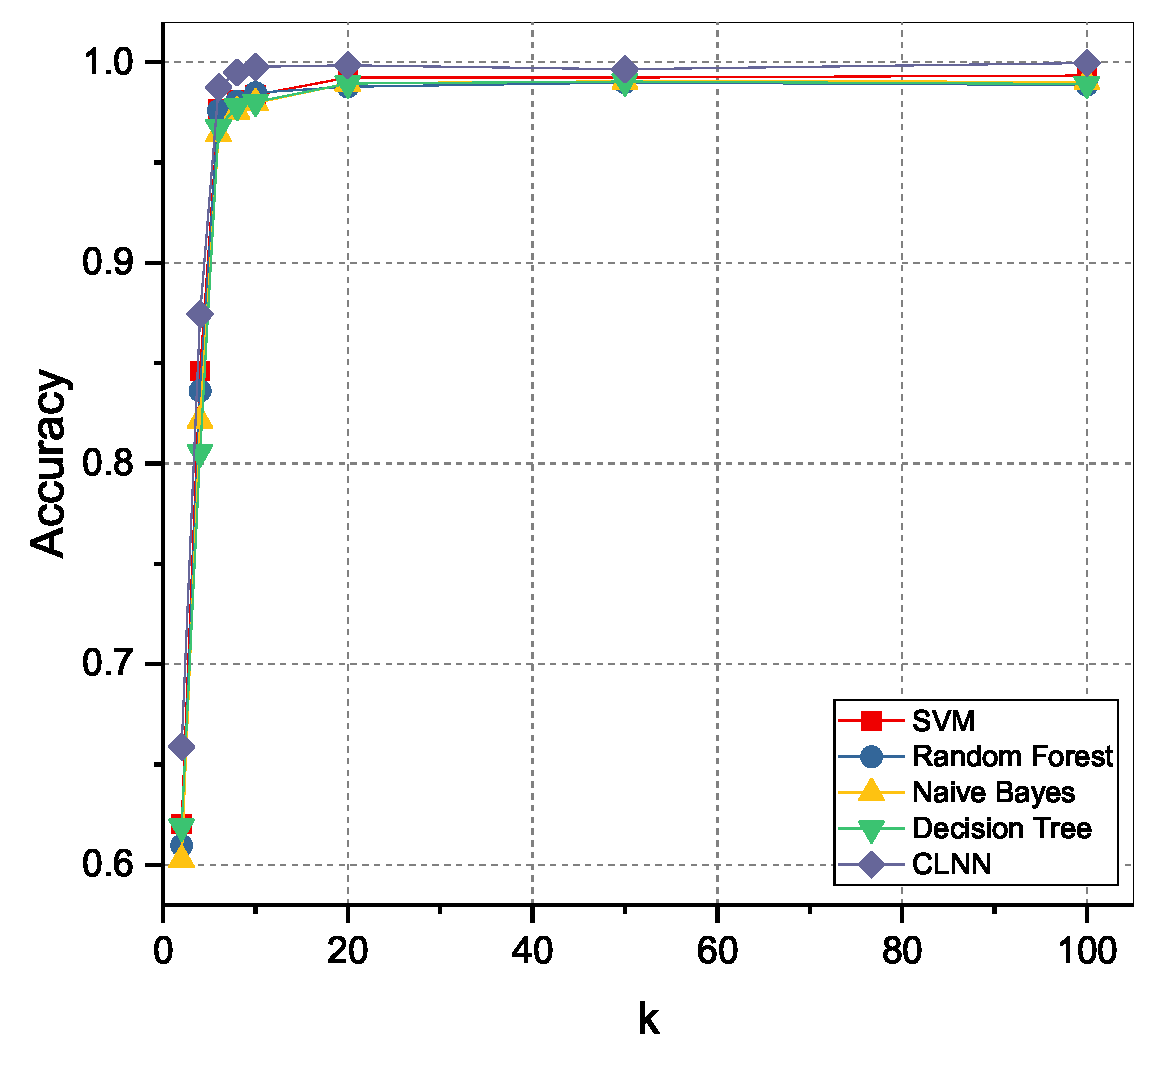
\includegraphics[width=0.8\textwidth]{figures/ml.eps}
  \caption{CLNN模型提取特征集与文章\supercite{5}中特征集对比}
  \label{fig:ml}
\end{figure}
\subsection{其他方法对比}


\section{实时性评估}
为了验证本文搭建的VoIP流量实时识别系统的实时性,本文使用数据集2模拟真实网络环境中的流量进行实时性验证。我们使用tcpreplay软件回放所收集到的VoIP流量,tcpreplay可以将我们收集到的pcap文件进行回放,并且其支持在回放的过程中修改网络层报头。我们通过tcpreplay工具在流量纯净的网卡上进行回放工作,我们记录从收到VoIP流的第一包到识别出结果所耗费的时间。表格\ref{tab:time4folws}展示了实时识别系统识别100个VoIP流所耗费的时间。可以看到,当我们使用k值为100的分类器进行识别平均识别每个流需耗费3秒钟,使用k值为2的分类器耗费0.3秒钟。对于不同情形下的识别需求,网络管理员可以按需对识别结果作出应对。

\begin{table}
  \caption{VoIP实时识别系统识别100个流所耗费的时间}
  %\caption{The time consumed to identify 100 flows.}
  \label{tab:time4folws}
  \centering
  \begin{tabular}{l l l l l l l }
    \hline
    \textbf{Model} &\textbf{k=6}&\textbf{k=8}&\textbf{k=10}&\textbf{k=20}&\textbf{k=40}&\textbf{k=100}\\
    \hline
    时间(s)      &29.09&30.53&48.00&73.62&141.33&309.51  \\
    \hline
  \end{tabular}
\end{table}

\section{本章小结}
本章首先介绍了CLNN模型的训练环境和VoIP流量实时识别系统的运行环境,之后对训练数据集和深度学习所使用的参数做了详细介绍。然后针对CLNN模型的识别性能从不同的层面做了评估,证明了CLNN模型的有效性。其次,我们还将本文所提出的方法与其他文章中的识别方法做了比较。最后,本文对VoIP流量实时识别系统的实时性作了评估。



\chapter{总结与展望}
VoIP应用的广泛使用势必会造成诸多的社会问题,为了使VoIP应用是可控的,对于VoIP应用流量的有效监管是必要的。由于VoIP应用的加密性和P2P的特性,VoIP流量的识别难度要远远高于其他流量的识别。本文总结整理了现存的VoIP流量识别方法,并分析了这些方法的优缺点。在此基础上,我们针对VoIP应用媒体传输流量进行了分析,设计了可以自动提取媒体传输流量的CLNN模型,该模型可以从时域和频域两个维度上最大限度的提取其特征用于VoIP识别。其次,本文提出了针对VoIP子流的实时识别方法,设计了可以应用于大规模真实网络的VoIP流量实时识别系统。同时,我们对于文中使用的各种方法进行了实验验证,证明了方法的可靠性。

\section{论文总结}

本文的主要工作如下:
1)本文研究了VoIP流量识别的关键技术。对于VoIP流量识别方法分为多个层次进行了介绍,分析了每种方法的针对点和适用性范围。

2)本文研究了与VoIP流量识别相关的各方面的知识。包括VoIP相关技术、流分类、深度学习等多个方面的内容,在此基础上,本文分析了VoIP流量所携带的各种可能用于进行识别的特征。之后结合卷积神经网络和长短期记忆网络模型在时域频域方面的建模能力,设计了可以自动提取VoIP流量特征的网络模型。本文同时在VoIP识别实时性方面作出要求,设计了基于子流进行识别的方法。结合深度学习方面的能力,该模型在保证识别精度的同时也保证了识别要求的实时性。

3)针对本文所提出的方法,我们设计了并实现了一个可以应用于大规模真实网络的VoIP流量实时识别系统。该系统采用Storm作为其流计算引擎,Kafka作为其负载均衡系统,保证了在大规模真实网络中的识别性能。在VoIP识别系统中引入了CLNN模型作为分类器,该分类器保证了对VoIP流量的识别精度。其次,我们对实时识别的性能通过加入VoIP流过滤器进行提升,从而提高了识别系统的实时性能。



\section{问题和展望}
本文提出的VoIP流量实时识别的方法在准确率和实时性方面都表现出了良好的性能,同时也可以部署到大规模的真实网络环境中。但是其中也存在一些问题,这些问题将作为我们进一步的研究内容:

1)本文实验中采集的数据集不够广泛,只能针对10种类别的VoIP应用流量进行识别,其次非VoIP应用的流量覆盖也不够广泛,对于未知的流量类型并没有一个良好的解决办法。在现在的实时系统中仅仅依靠识别结果的概率分布进行判断。下一步我们需要增加VoIP应用和非VoIP流量的种类,并且进一步扩大训练数据集,使得CLNN模型识别性能更加稳健。

2)使用深度学习进行训练所要求的庞大的数据集导致训练时间过长。当我们尝试向需要识别的VoIP流量中新增一种新的类型,当前我们不得不重新训练数据集来获得CLNN分类器,这就造成了不必要的训练过程。构建VoIP应用种类足够充足的数据集当然是解决此问题的最优方法,但是为了防止扩展VoIP类型带来的种种消耗,我们仍需研究新方法解决该问题。

%3)




%% -*- coding: utf-8 -*-

% -*- coding: utf-8 -*-

\def\bibrangedash{ $\sim$ }
\printbibliography [ category = cited]


\listoffigures
%\clearpage
%{\phantomsection
\listoftables
% -*- coding: utf-8 -*-

%\makeschapterhead{致谢}
\chapter*{致谢}
感谢您使用本模板。

% -*- coding: utf-8 -*-


\chapter*{个人简历}

\end{document}
